\documentclass{article}

% if you need to pass options to natbib, use, e.g.:
    \PassOptionsToPackage{numbers, compress}{natbib}
% before loading neurips_2018

% ready for submission
% \usepackage{neurips_2018}

% to compile a preprint version, e.g., for submission to arXiv, add add the
% [preprint] option:
\usepackage[preprint]{nips_2018}

% to compile a camera-ready version, add the [final] option, e.g.:
     %\usepackage[final]{neurips_2018}

% to avoid loading the natbib package, add option nonatbib:
%     \usepackage[nonatbib]{neurips_2018}

\usepackage[utf8]{inputenc} % allow utf-8 input
\usepackage[T1]{fontenc}    % use 8-bit T1 fonts
\usepackage{hyperref}       % hyperlinks
\usepackage{url}            % simple URL typesetting
\usepackage{booktabs}       % professional-quality tables
\usepackage{amsfonts}       % blackboard math symbols
\usepackage{nicefrac}       % compact symbols for 1/2, etc.
\usepackage{microtype}      % microtypography
\usepackage{natbib}
\usepackage{color}
\usepackage{amsmath}
\usepackage{amsthm}
\usepackage{graphicx}
\usepackage[ruled]{algorithm2e}
\usepackage{bbm}
\usepackage{subcaption}
\usepackage{caption}
\usepackage{array}
\newcolumntype{P}[1]{>{\centering\arraybackslash}p{#1}}

\SetKwInput{kwInit}{Init}
\newtheorem*{remark}{Remark}

\DeclareMathOperator*{\argmin}{arg\,min}
\DeclareMathOperator*{\argmax}{arg\,max}
\newtheorem{theorem}{Theorem}
%\newtheorem{theorem}{Theorem}[section]
\newtheorem{proposition}[theorem]{Proposition}
\newtheorem{lemma}{Lemma}
\newtheorem{corollary}[theorem]{Corollary}
\newtheorem{definition}[theorem]{Definition}
\newtheorem{assumption}[theorem]{Assumption}

\newcommand{\RSA}{\mathbb{R}^{|\mathcal{S}|\times|\mathcal{A}|}}
\newcommand{\RSAvector}{\mathbb{R}^{|\mathcal{S}||\mathcal{A}| \times 1}}
\newcommand{\RS}{\mathbb{R}^{|\mathcal{S}|}}
\newcommand{\Rvector}[1]{\mathbb{R}^{#1}}
\newcommand{\Rmatrix}[2]{\mathbb{R}^{#1 \times #2}}
\newcommand{\AdaBracket}[1]{\left(#1\right)}
\newcommand{\AdaRectBracket}[1]{\left[#1\right]}
\newcommand{\AdaAngleBracket}[1]{\left\langle#1\right\rangle}
\newcommand{\AdaAngleProduct}[2]{\left\langle#1, #2\right\rangle}
\newcommand{\chiAny}[3]{\chi^{#1}\AdaBracket{#2||#3}}
\newcommand{\expectation}[2]{\mathbb{E}_{#1}\AdaRectBracket{#2}}
\newcommand{\qlog}{$q$-logarithm }
\newcommand{\qexp}{$q$-exponential }
\newcommand{\fdiv}{$f$-divergence }
\newcommand{\qstarlog}{$q^*$-logarithm }
\newcommand{\qstarexp}{$q^*$-exponential }
\newcommand{\tsallis}[1]{S_q(#1)}
\newcommand{\sparse}[1]{S_2(#1)}
\newcommand{\qKL}{D^{q}_{\!K\!L}\!\AdaBracket{\pi || \bar{\pi}}}
\newcommand{\qKLindex}[2]{D^{q}_{\!K\!L}\!\AdaBracket{\pi_{#1}|| \pi_{#2}}}
\newcommand{\qstarKLindex}[2]{D^{q^*}_{\!K\!L}\!\AdaBracket{\pi_{#1}|| \pi_{#2}}}
\newcommand{\qKLany}[2]{D^{q}_{\!K\!L}\!\left(#1 \left|  \right| #2 \right)}
\newcommand{\qKLstarany}[2]{D^{q^*}_{\!K\!L}\!\left(#1 \left|  \right| #2 \right)}
\newcommand{\KL}{D_{\!K\!L}\!\AdaBracket{\pi || \bar{\pi}}}
\newcommand{\KLindex}[2]{D_{\!K\!L}\!\AdaBracket{\pi_{#1}|| \pi_{#2}}}
\newcommand{\KLany}[2]{D_{\!K\!L}\!\left(#1 \left|  \right| #2 \right)}
\newcommand{\entropy}{\mathcal{H}\left( \pi \right)}
\newcommand{\entropyany}[1]{\mathcal{H}\left( #1 \right)}
\newcommand{\entropyIndex}[1]{\mathcal{H}\left( \pi_{#1} \right)}
\newcommand{\fdivany}[2]{D_{f}\!\left(#1 \left|  \right| #2 \right)}
\newcommand{\logq}[1]{\ln_{q}\!#1}
\newcommand{\logstarq}[1]{\ln_{q^*}\!#1}
\newcommand{\expq}[1]{\exp_{q}\!#1}
\newcommand{\expstarq}[1]{\exp_{q^*}\!#1}
\newcommand{\eq}[1]{Eq.\,(#1)}
\newcommand{\taulogqratio}[3]{\mathbb{M}_{#1,#2} + \ln_{#3}{\pi}_{#1}}
\newcommand{\uniformA}{\left|\mathcal{A}\right|}
\newcommand{\normalization}[1]{\tau\psi\AdaBracket{ \frac{Q_{#1}}{\tau}}}
\newcommand{\renyi}{Rényi }
\newcommand{\renyidivany}[2]{D_\text{\renyi}\!\!\AdaBracket{ #1 || #2}}
\newcommand{\transition}{\gamma P_{\pi}}
\newcommand{\greedy}[1]{\argmax_{\pi}\!\AdaAngleProduct{\pi}{#1}}
\newcommand{\greedyH}[1]{\argmax_{\pi}\!\AdaAngleProduct{\pi}{#1 - \tau\ln\pi}}
\newcommand{\greedyOmega}[1]{\argmax_{\pi}\!\AdaBracket{\AdaAngleProduct{\pi}{#1} - \tau\Omega(\pi)}}
\newcommand{\greedyTKL}[1]{\argmax_{\pi}\!\AdaAngleProduct{\pi}{#1 - \ln_{{q}}\!\frac{\pi}{\pi_k}}}
\newcommand{\BellmanKL}[2]{T^{\lambda,0}_{\pi_{#1}|\pi_{#2}}}
\newcommand{\BellmanKLGreek}[3]{T^{#1,0}_{\pi_{#2}|\pi_{#3}}}
\newcommand{\BellmanKLbar}{T^{\lambda, 0}_{\pi|\bar{\pi}}}
\newcommand{\BellmanH}[2]{r + \gamma P\!\AdaAngleProduct{\pi_{#1}}{Q_{#2} -
\tau\ln\pi_{#1}}}
\newcommand{\BellmanOmega}[2]{r + \gamma P\!\AdaBracket{ \AdaAngleProduct{\pi_{#1}}{Q_{#2}} - \tau\Omega(\pi_{#1})}}
\newcommand{\BellmanTKL}[2]{r + \gamma P\!\AdaAngleProduct{\pi_{#1}}{\TsallisQ{#2} - \ln_{q}\!\frac{\pi_{#1}}{\pi_{#2}}}}
\newcommand{\BellmanImplicit}[2]{\tilde{T}^{0,#1}_{\pi_{#2}}}
\newcommand{\BellmanBoth}[4]{{T}^{#1,#2}_{\pi_{#3}|\pi_{#4}}}
\newcommand{\BellmanG}[1]{T^{\alpha}_{\pi_{#1}}}
\newcommand{\Bellman}[1]{r + \gamma P_* Q_{#1} }
\newcommand{\sumJK}[1]{\sum_{j=#1}^{k}}
\newcommand{\datasetQ}{Q_{\pi_{\mathcal{D}}}}
\newcommand{\datasetOptimalQ}{Q_{*, \pi_{\mathcal{D}}}}
\newcommand{\datasetPolicy}{\pi_{\mathcal{D}}}


\title{Offline Reinforcement Learning with In-Sample Tsallis Regularized Policy}

% The \author macro works with any number of authors. There are two commands
% used to separate the names and addresses of multiple authors: \And and \AND.
%
% Using \And between authors leaves it to LaTeX to determine where to break the
% lines. Using \AND forces a line break at that point. So, if LaTeX puts 3 of 4
% authors names on the first line, and the last on the second line, try using
% \AND instead of \And before the third author name.

\author{%
  Department of Computing Science\\
  Alberta University\\
  Pittsburgh, PA 15213 \\
  \texttt{hippo@cs.cranberry-lemon.edu} \\
  % examples of more authors
  % \And
  % Coauthor \\
  % Affiliation \\
  % Address \\
  % \texttt{email} \\
  % \AND
  % Coauthor \\
  % Affiliation \\
  % Address \\
  % \texttt{email} \\
  % \And
  % Coauthor \\
  % Affiliation \\
  % Address \\
  % \texttt{email} \\
  % \And
  % Coauthor \\
  % Affiliation \\
  % Address \\
  % \texttt{email} \\
}

\begin{document}
% \nipsfinalcopy is no longer used

\maketitle

\begin{abstract}
    Offline reinforcement learning methods learn from a fixed dataset collected by some behavior policy without further interaction with the environment.
    Such datasets often contain only a subset of the state and action spaces. 
    Standard off-policy algorithms suffer from the extrapolation error known as the  unrealistic action values for the actions not present in the dataset.
    The inaccurate value estimate can in turn cause out-of-distribution actions to be preferred in the policy improvement stage, leading to poor performance.
    Many methods propose to enforce the closedness between the learned policy and the behavior policy.
    In this paper, we propose to learn a in-sample Tsallis regularized policy that has support strictly within the dataset support. 
    Our method also generalizes the in-sample softmax as a special case of the Tsallis policy where the support of the learned policy remains the same to the behavior policy.
    Moreover, if we assume the dataset is generated by Tsallis policies such that the absent actions are truncated, then we can guarantee the learned Tsallis policy is sufficiently similar to the behavior policy by showing bounded KL distance.
    This is the firs application of Tsallis regularization to offline RL to the best of our knowledge, where insufficient exploration as one of the main drawbacks of Tsallis regularized policies vanishes.
    
\end{abstract}


\section{Introduction}





\section{Background}

\subsection{Reinforcement Learning}

We focus on discrete-time discounted Markov Decision Processes (MDPs) expressed by the tuple $(\mathcal{S}, \mathcal{A}, P,  r,  \gamma)$, where $\mathcal{S}$ and $\mathcal{A}$ denote state space and finite action space, respectively. 
% $d(\cdot)$ denotes the initial state distribution.
$P(\cdot |s,a)$ denotes transition probability over the state space given state-action pair $(s,a)$,  
and $r(s,a)$ defines the reward associated with that transition. 
$\gamma \in (0,1)$ is the discount factor.
A policy $\pi(\cdot|s)$ is a mapping from the state space to distributions over actions.
% The stationary state distribution induced by $\pi$ can then be defined as $d^{\pi}_{\mu}(s)\!:=\!(1-\gamma)\sum^{\infty}_{t=0}\gamma^{t}P(s_t=s|\pi, \mu)$.
% We define the state value function at a specific state $s$ following policy $\pi$  as  $V_{\pi}(s) = \mathbb{E}\AdaRectBracket{\sum_{t=0}^{\infty} r_t | s }$.
The state-action value function starting from $(s, a)$ following policy $\pi$ is defined as  $Q_{\pi}(s,a) = \mathbb{E}_{\pi}\AdaRectBracket{\sum_{t=0}^{\infty} \gamma^t r(s_t, a_t) | s_0=s, a_0 = a }$.
It is a classic result that there exists a stationary optimal policy that maximizes the cumulative return \cite{Puterman1994}.
Its fixed point $Q_{*}(s,a)$ satisfies the Bellman optimality equation $Q_{*}(s,a) = r(s,a) + \gamma  \mathbb{E}_{s'\sim P(\cdot|s,a)}\!\AdaRectBracket{\max_{a'}Q_*(s',a')}$.
Therefore, in practice it is common to update the action value function by acting greedily with respect to the current estimate.


We are interested in the MDPs that are \emph{entropy-regularized}: the reward function is augmented with an additional entropic penality (or bonus).
For example, the Shannon entropy $\entropyany{\pi(\cdot| s)} := -\sum_a \pi(a|s)\ln \pi(a|s)$ is often added as a bonus to encourage the policy to be stochastic.
The maximum Shannon entropy action value function satisfies $\tilde{Q}_{\pi}(s,a) = r(s,a) + \gamma \mathbb{E}_{s' \sim P(\cdot | s,a )}\mathbb{E}_{a\sim \pi(\cdot|s)}\AdaRectBracket{\tilde{Q}_{\pi}(s,a) - \tau\entropyany{\pi(\cdot|s)}}$, where $\tau$ denotes a coefficient.
The maximum $r(s,a) + \gamma \expectation{s'\sim P(\cdot|s,a)}{\tau \ln\sum_{a} \exp\AdaBracket{\tau^{-1}Q_{\pi}(s,a)}}$ is attained when the policy is the well-known Boltzmann softmax $\pi(a|s) \propto \exp\AdaBracket{\tau^{-1}Q_{\pi}(s,a)}$, where $\propto$ denotes proportional to up to a constant not depending on actions.
KL divergence $\KLany{\pi(\cdot|s)}{\mu(\cdot|s)}:= \sum_a \pi(a|s)\ln\frac{\pi(a|s)}{\mu(a|s)}$ is another popular choice, where $\mu$ is some baseline policy \cite{azar2012dynamic,Rawlik2013-SOCRL,vieillard2020leverage}.
Unlike Shannon entropy, KL divergence is often added as a penalty to penalize large deviation from $\mu$.
The KL-regularized optimal policy takes the form $\pi(a|s) \propto \mu(a|s)\exp\AdaBracket{\tau^{-1}Q_{\pi}(s,a)}$, where we overloaded the coefficient $\tau$ for Shannon entropy.

% \begin{align}
%     Q_{\pi}(s,a) = \mathbb{E}\AdaRectBracket{\sum_{t=0}^{\infty} r_t | s_0=s, a_0 = a } ,
% \end{align}
% where the expectation is with respect to the policy $\pi$ and transition probability $P$.
% A standard approach to find the optimal value function $Q_*$ is value iteration. To define the formulas for value iteration, it will be convenient to write these functions as vectors, $V_{\pi} \in \RS$ and $Q_{\pi} \!\in\! \RSA$. 
% For notational convenience, we define the inner product for any two functions $F_1,F_2\in\RSA$  as $\AdaAngleProduct{F_1}{F_2} \in \RS$, where we only take the inner product over actions. 
% % MARTHA: mention this when it is used
% %$\boldsymbol{1}$ denotes an all-one vector whose dimension should be clear from the context.
% The Bellman operator acting upon any function $Q \!\in\! \RSA$ can be defined as: $T_{\pi}Q := r + \transition Q$, where $P_{\pi}Q \!\in\! \RSA \!:=\! \mathbb{E}_{s'\sim P(\cdot|s,a),a'\sim\pi(\cdot|s')}\!\AdaRectBracket{Q(s',a')} \!=\! P\!\AdaAngleProduct{\pi}{Q}$.
% When $\pi$ is greedy with respect to $Q$, we have the Bellman optimality operator defined by $T_*Q := r + \gamma P_* Q$, $P_*Q \!=\! \mathbb{E}_{s'\sim P(\cdot|s,a)}\!\AdaRectBracket{\max_{a'}Q(s',a')}$. 
% The above definitions should be understood as component-wise.
% Repeatedly applying the Bellman operator $T_{\pi}Q$ converges to the unique fixed point $Q_{\pi}$, and $T_*Q$ it converges to the optimal action value function $Q_*:=Q_{\pi^*}$.
% % Typically the Bellman operator is applied $m \geq 1$ times, and
% % $m=1,\infty$ corresponds value iteration and policy iteration, respectively.
% % $1\!<\! m < \!\infty\!$ implies the use of approximate modified policy iteration \citep{scherrer15-AMPI}.
% This basic recursion can be modified with the addition of a regularizer $\Omega(\pi)$:
% \begin{align}
%     \begin{cases}
%         \pi_{k+1} = \greedy{Q_{k}}, & \\
%         Q_{k+1} =  \AdaBracket{ T_{\pi_{k+1}} Q_k }^m , &
%     \end{cases}
%     \label{eq:PI}
% \quad
%     \begin{cases}
%         \pi_{k+1} = \greedyOmega{Q_{k}}, & \\
%         Q_{k+1} = \AdaBracket{T_{\pi_{k+1, \Omega}}Q_k}^m &
%     \end{cases}
% \end{align}
% % MARTHA: What? why would m = infty be policy iteration? this formulas has T_*
% %
% % \begin{align}
% %   \begin{cases}
% %       \pi_{k+1} = \greedyOmega{Q_{k}}, & \\
% %       Q_{k+1} = \AdaBracket{T_{\pi_{k+1, \Omega}}Q_k}^m &
% %   \end{cases}
% %   \label{eq:regularizedPI}
% % \end{align}
% where $T_{\pi_{k+1}, \Omega}Q_k \!=\! \BellmanOmega{k+1}{k}$ is the regularized Bellman operator \citep{geist19-regularized}. This modified recursion is guaranteed to converge if $\Omega$ is concave in $\pi$. For standard (Shannon) entropy regularization, we use $\Omega(\pi) = -\entropy = \AdaAngleProduct{\pi}{\ln\pi}$. The resulting optimal policy has $\pi_{k+1} \propto \exp\AdaBracket{\tau^{-1}Q_k}$, where $\propto$ indicates \emph{proportional to} up to a constant not depending on actions.

% Another popular choice is KL divergence $\Omega(\pi)=\KLany{\pi}{\mu} = \AdaAngleProduct{\pi}{\ln{\pi} \!-\!\ln{\mu}}$, which is more general since we recover Shannon entropy when we choose $\mu$ to be a uniform distribution, i.e. $\frac{1}{|\mathcal{A}|}$. In this work, when we say KL regularization, we mean the standard choice of setting $\mu = \pi_k$, the estimate from the previous update.
% Therefore, $D_\text{KL}$ serves as a penalty to penalize aggressive policy changes.
% The optimal policy in this case takes the form $\pi_{k+1}\propto\pi_k\exp\AdaBracket{\tau^{-1} Q_k}$.
% By induction, we can show this KL-regularized optimal policy $\pi_{k+1}$ is a softmax over a uniform average over the history of action value estimates \cite{vieillard2020leverage}:
% \begin{align}
%   \pi_{k+1} \propto \pi_k \exp\AdaBracket{\tau^{-1} Q_k}  \propto \cdots \propto \exp\AdaBracket{\! \tau^{-1}\sumJK{1}Q_j}
%   .
%   \label{eq:average}
% \end{align}
% Using KL regularization has been shown to be theoretically superior to entropy regularization, in terms of error tolerance \cite{azar2012dynamic,vieillard2020leverage,Kozuno-2022-KLGenerativeMinMaxOptimal,chan2021-greedification}.

% The definitions of $\mathcal{H}(\cdot)$ and $D_\text{KL}(\cdot||\cdot)$ rely on the standard logarithm and its inverse (the exponential) and both induce softmax policies as an exponential over (weighted) action-values \citep{hiriart2004-convexanalysis,Nachum2020-RLFenchelRockafellar}. 
% Convergence properties of the resulting regularized algorithms have been well studied \citep{kozunoCVI,geist19-regularized,vieillard2020leverage}.
% In this paper, we investigate Tsallis entropy and Tsallis KL divergence as the regularizer, which generalize Shannon entropy and KL divergence respectively.

\subsection{$q$-statistics and Tsallis regularization}


\begin{figure}
    \centering
    \begin{subfigure}[b]{0.3\textwidth}
        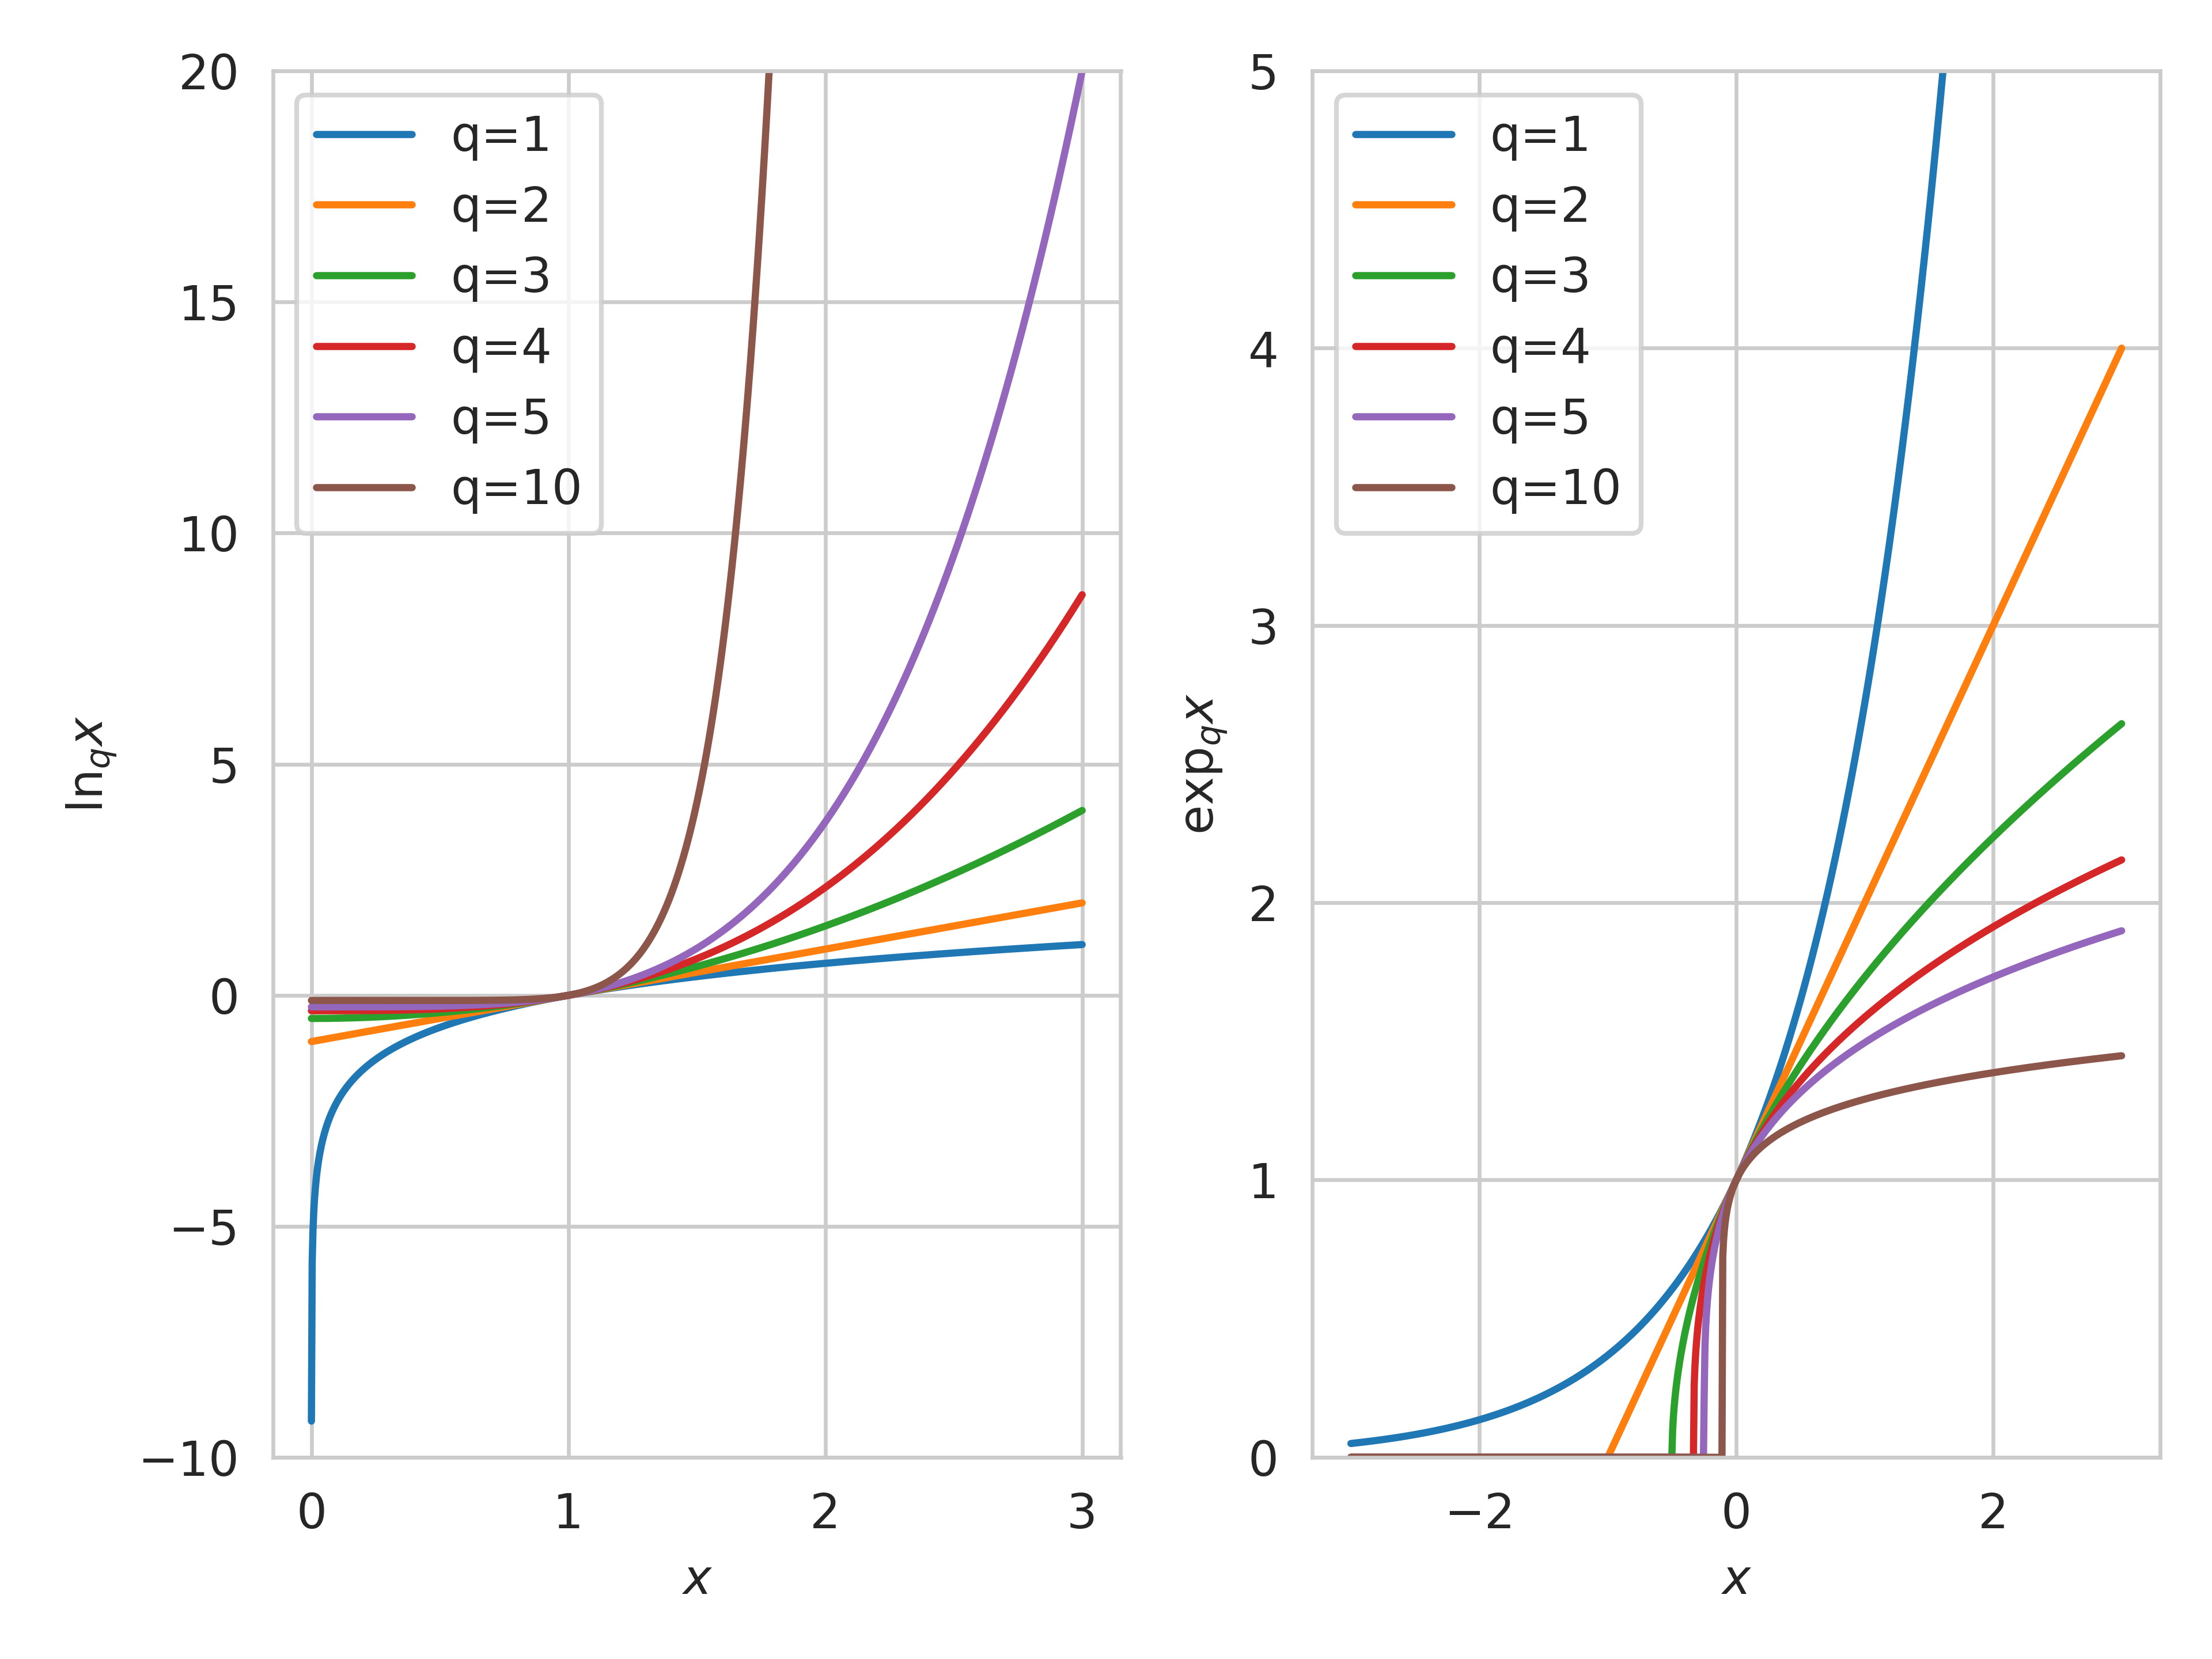
\includegraphics[width=\textwidth]{img/q_stat_illus.png}
    \end{subfigure}
    \begin{subfigure}[b]{0.3\textwidth}
        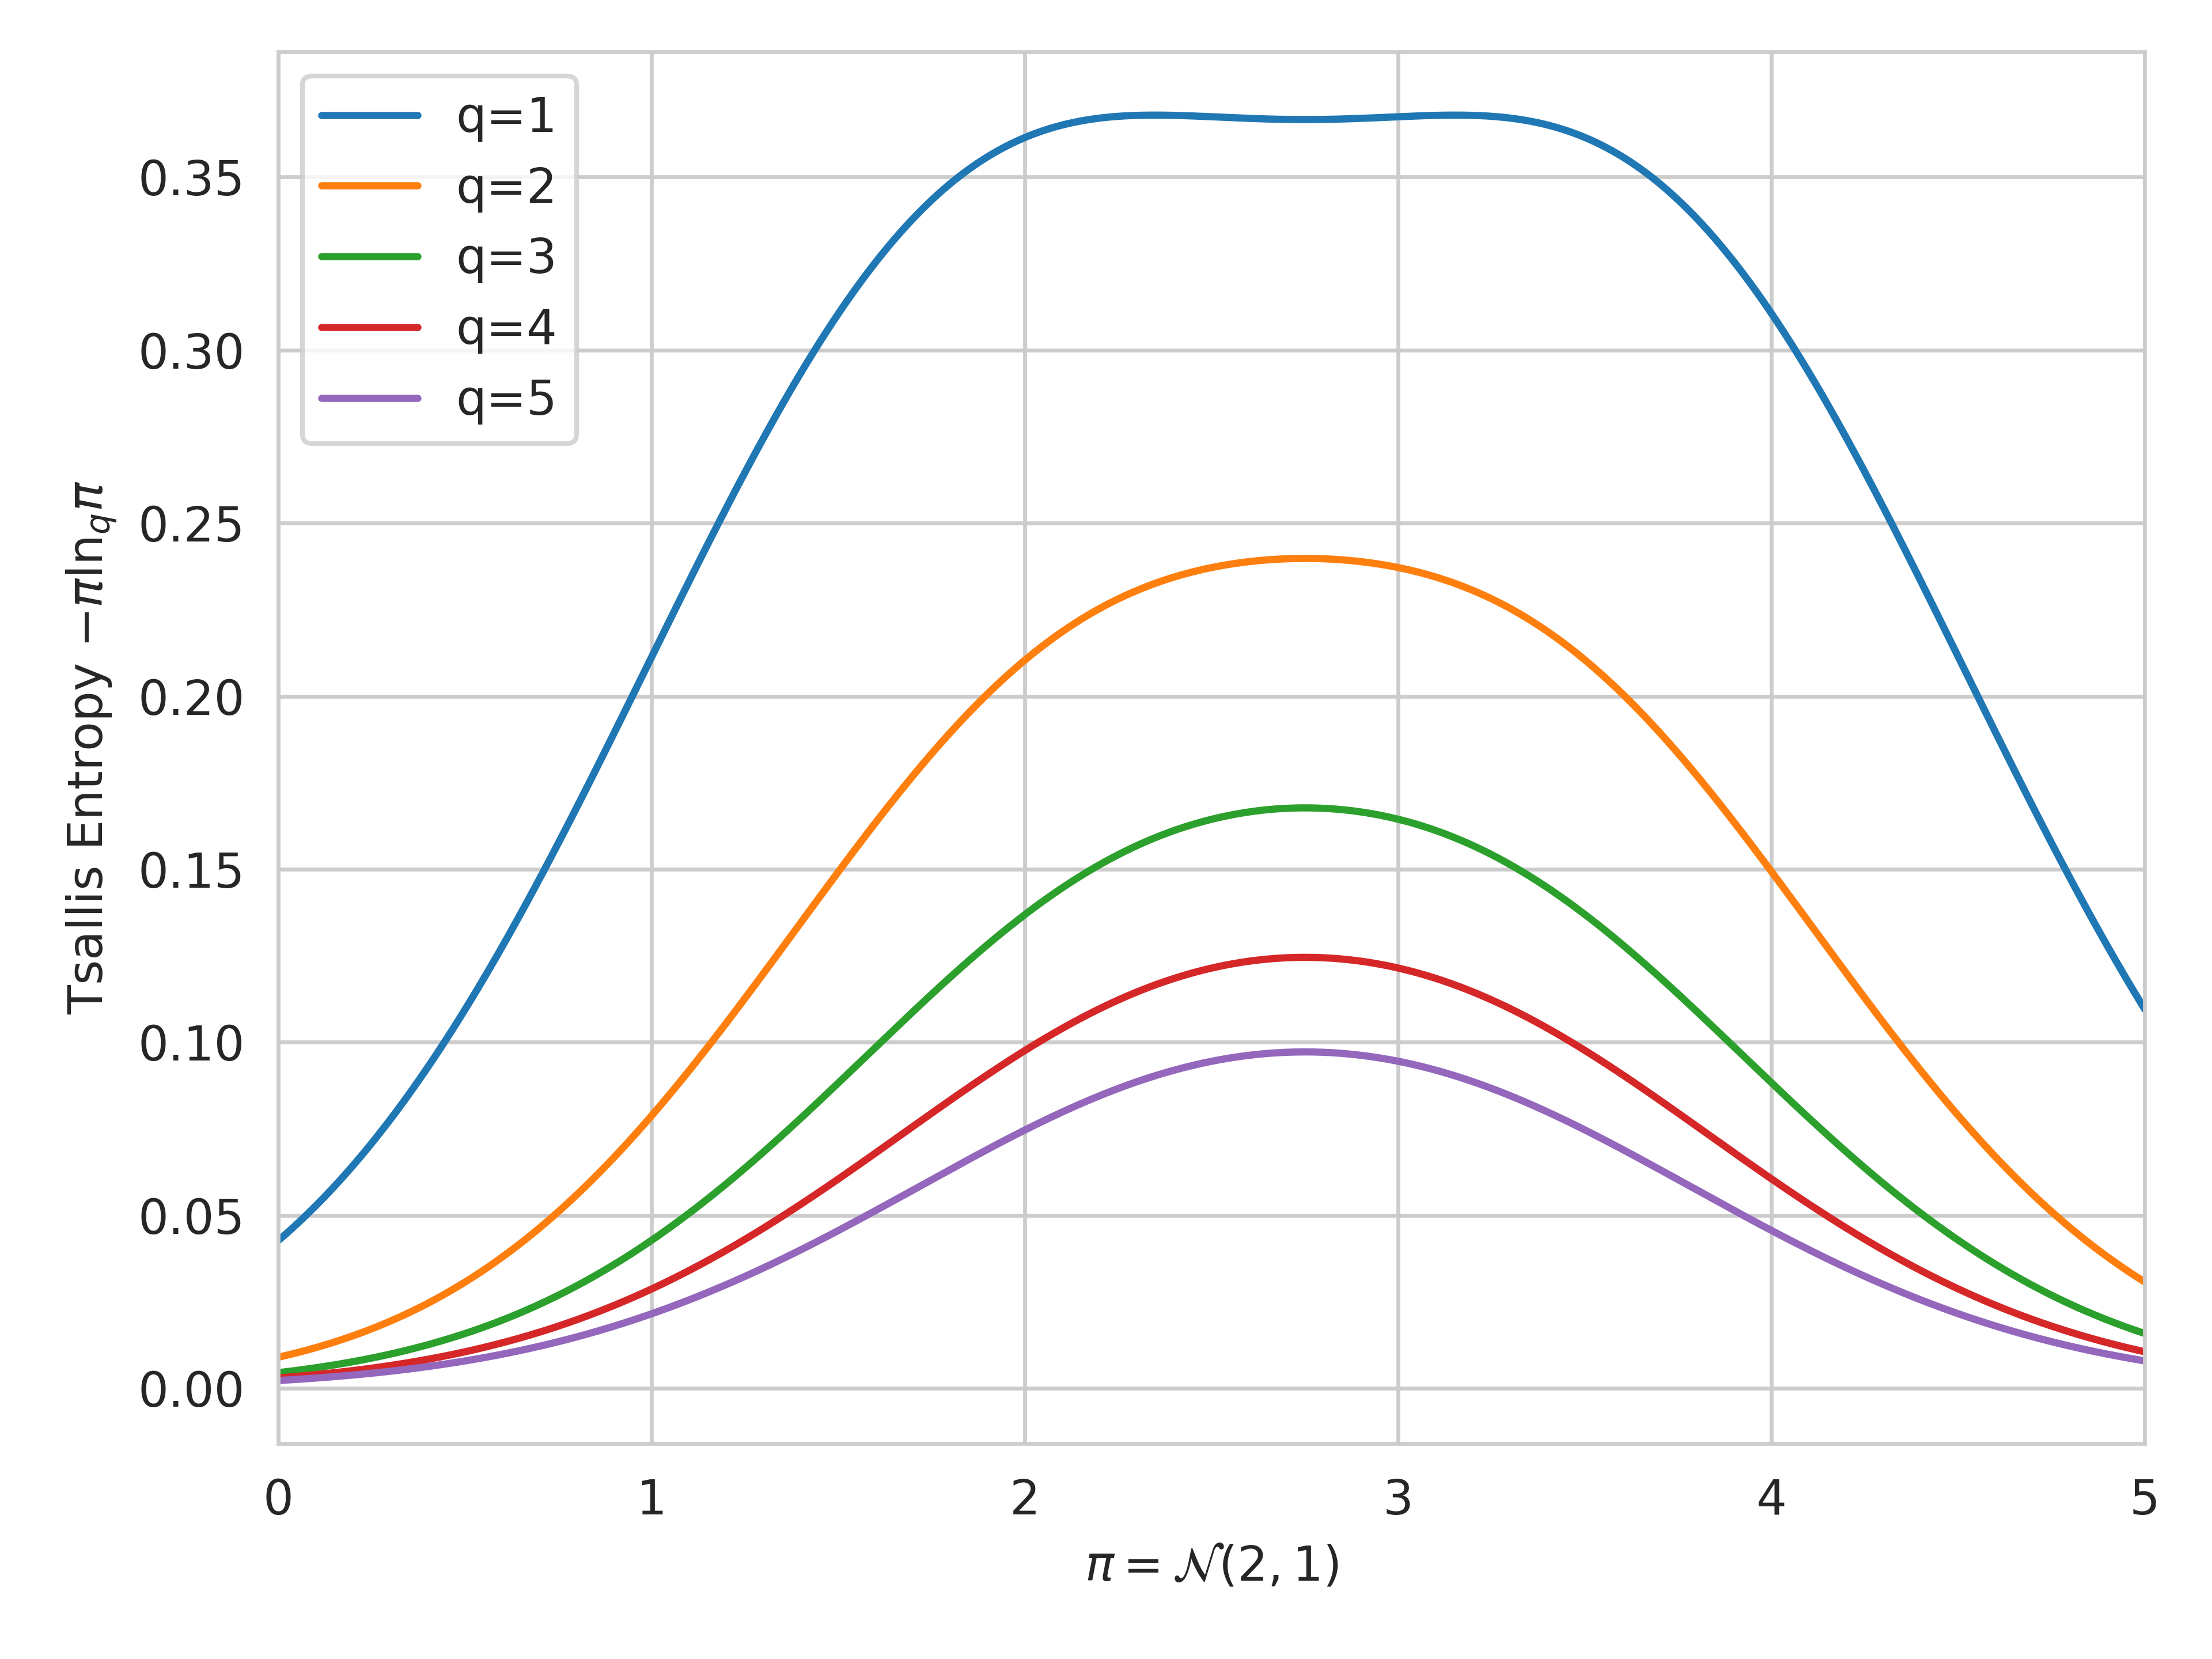
\includegraphics[width=\textwidth]{img/tsallis_entropy.png}
    \end{subfigure}
    \begin{subfigure}[b]{0.3\textwidth}
        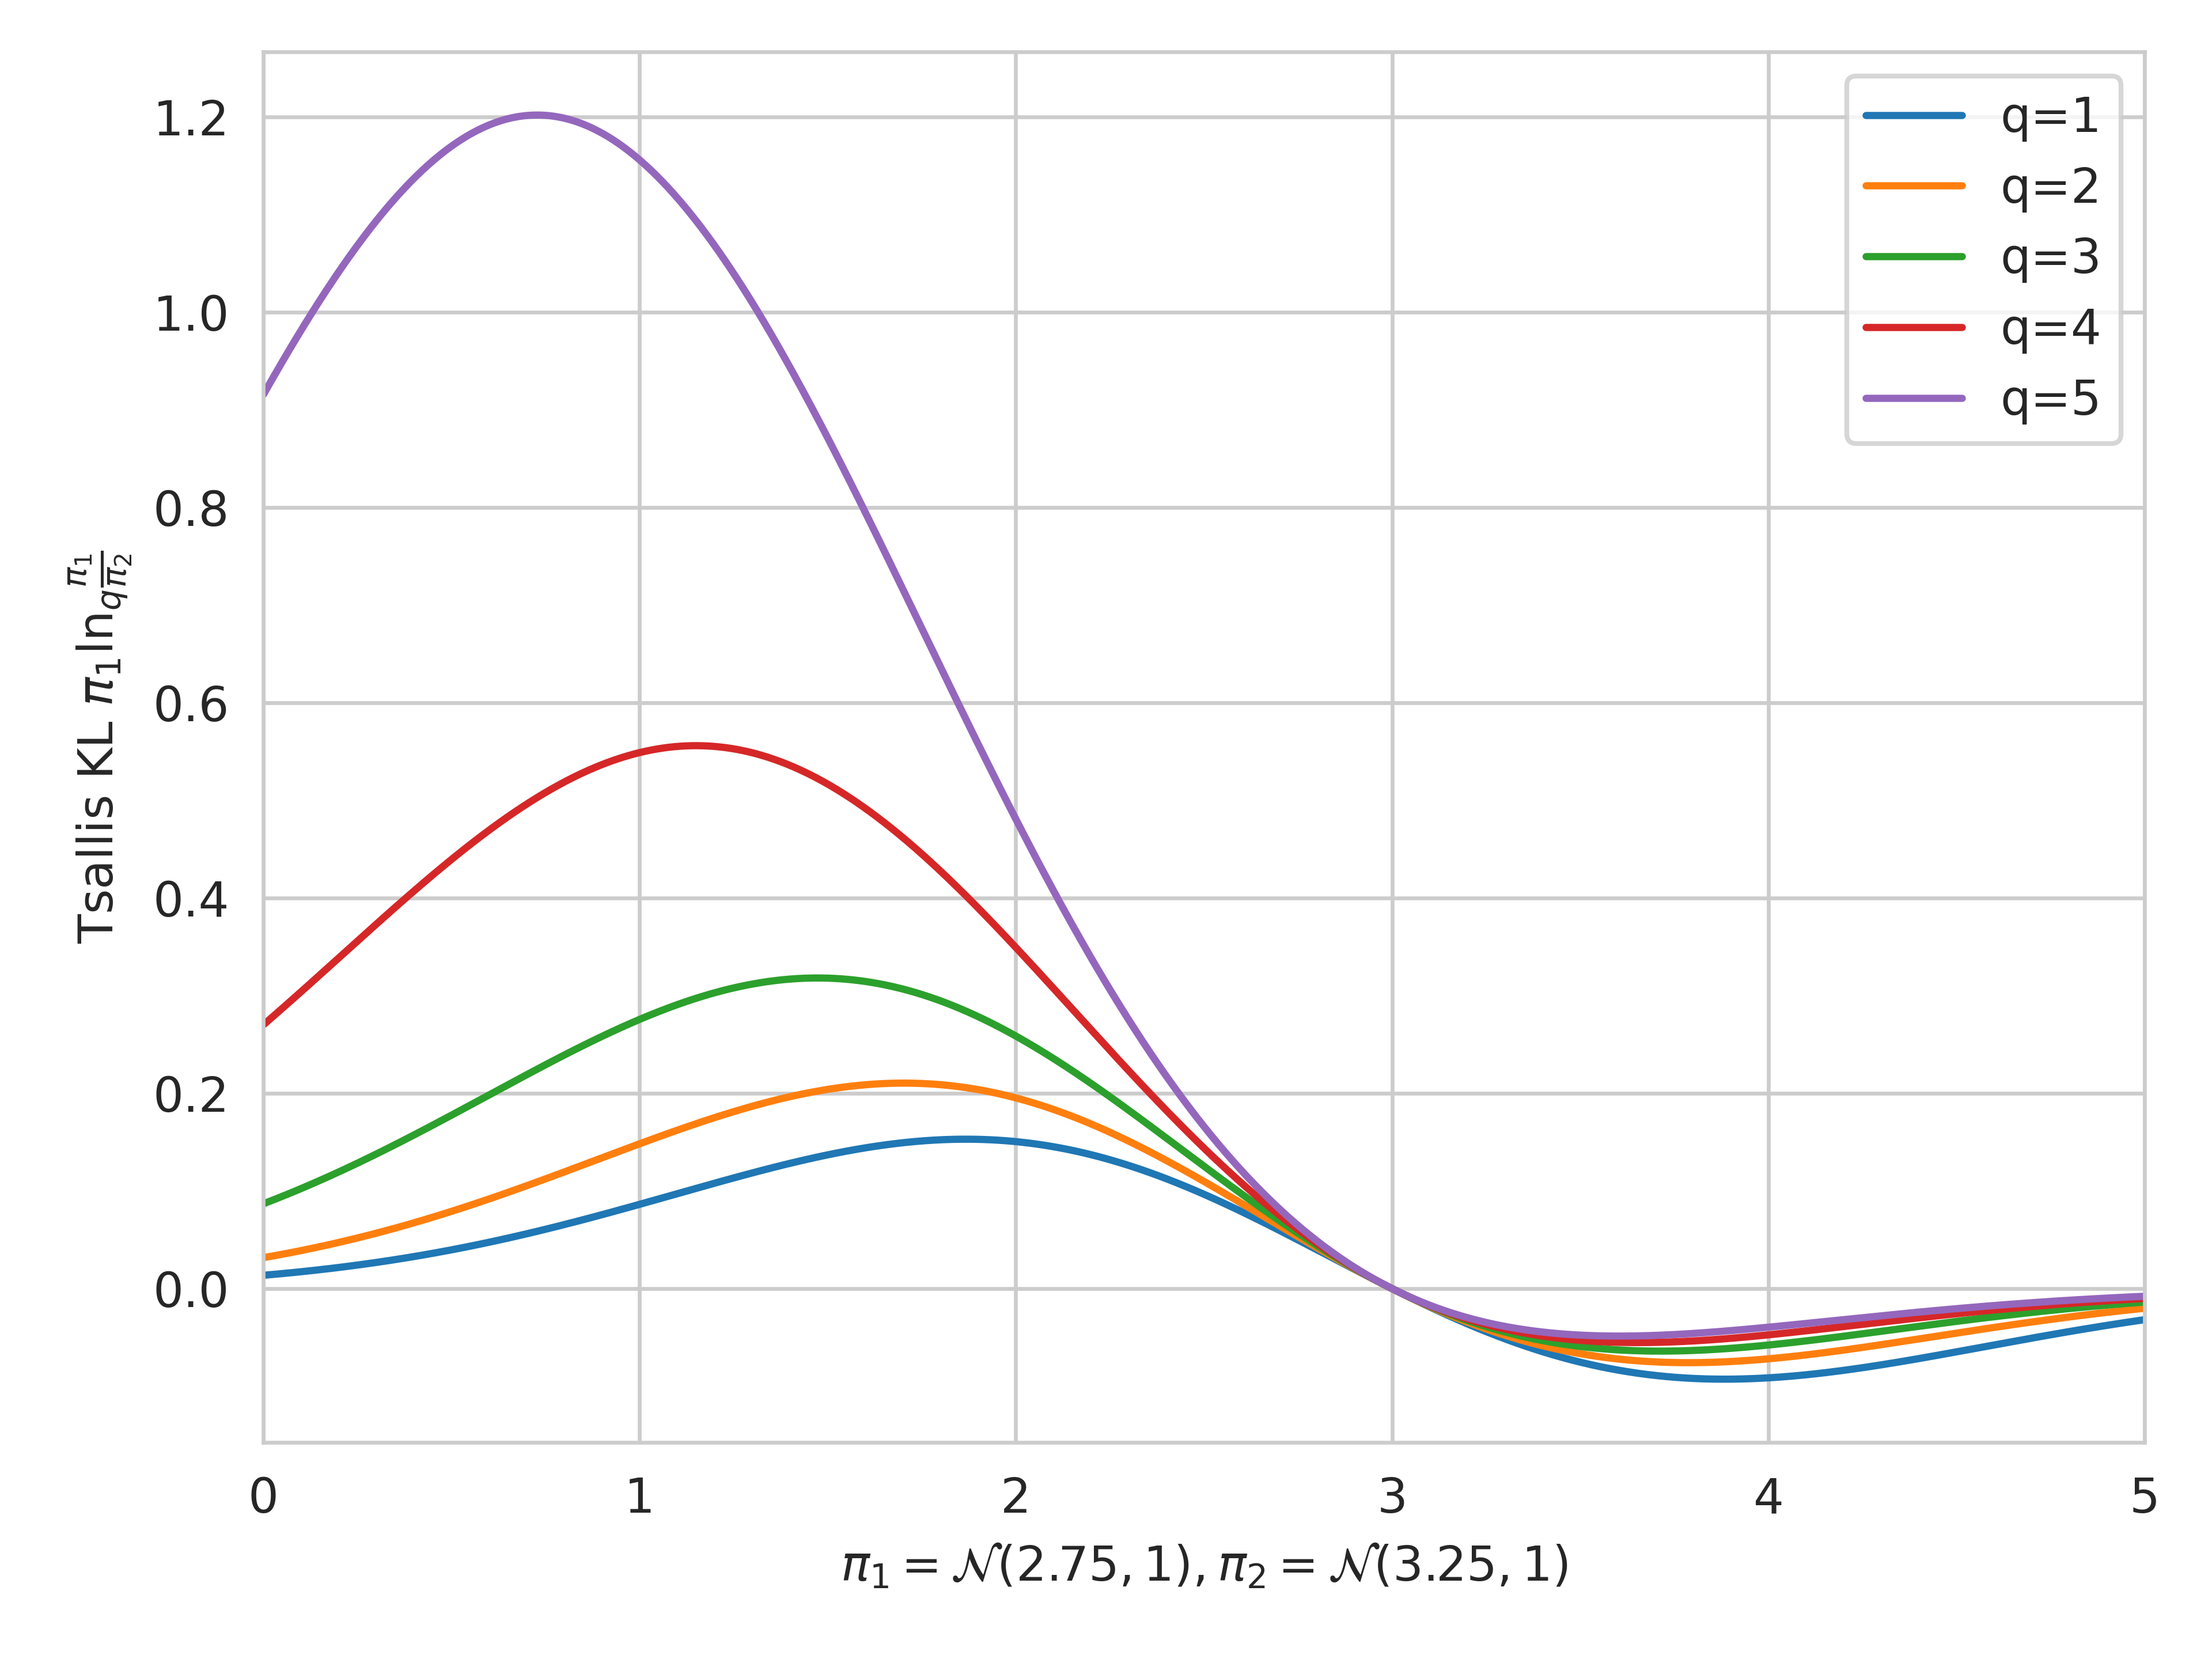
\includegraphics[width=\textwidth]{img/tsallis_kl.png}
    \end{subfigure}
    \caption{(Left) Behavior of \qlog and $q$-exponential functions.
    When $q=1$ they respectively recover the standard logarithm and exponential.
    (Mid) Tsallis entropy of the Gaussian policy $\mathcal{N}(2, 1)$. (Right) Tsallis KL divergence between two Gaussian policies $\mathcal{N}(2.75, 1)$ and $\mathcal{N}(3.25, 1)$.
    }
    \label{fig:q_stats}
\end{figure}

In this paper we consider a broad class of less studied entropic regularizer known as the Tsallis entropy $S_q(\pi(\cdot|s)):= \frac{1}{q-1} \AdaBracket{\sum_a \pi^q(a|s) - 1}$, where $q \in \mathbb{R}_{+}$.
It is also called generalized entropy since it generalizes the Shannon entropy \cite{TsallisEntropy,tsallis2009introduction}.
Tsallis entropy can also be defined by the \qlog in a similar manner to the standard logarithm defining Shannon entropy, hence eases the notation and derivation.
\qlog and its unique inverse function $q$-exponential are defined by \cite{tsallis2009introduction}:
\begin{align}
    \begin{split}
        \logq{x} = \frac{x^{q-1} - 1}{q-1}, \quad \expq{x} = \AdaRectBracket{1 + (q - 1)x}^{\frac{1}{q-1}}_{+}, \quad \tsallis{\pi(\cdot|s)} = -\sum_{a}{\pi(a|s)}{\logq{\pi(a|s)}},
    \end{split}
\end{align}
where $[\cdot]_{+} = \max \{\cdot, 0\}$.
When $q\rightarrow 1$, the \qlog (resp. $q$-exponential) recovers the standard logarithm (resp. exponential) and hence Tsallis entropy degenerates to Shannon entropy.
When $q=2$, we arrive at the Tsallis sparse entropy 
$S_2(\pi(\cdot | s)):= \pi(a|s)\AdaBracket{1 - \pi(a|s)}$ \cite{Nachum18a-tsallis,Lee2018-TsallisRAL}. 
The name sparse entropy comes from the fact that the regularizer leads to sparse support for the resulting policy \cite{Blondel-2020LearningFenchelYoundLoss,Martins16-sparsemax}.
When $q=\infty$, the regularizer vanishes.
In Figure \ref{fig:q_stats} we plot the behavior of $q$-statistics under different $q$.

We can write out the regularized policy for general Tsallis entropy regularization for any $q$\footnotemark\footnotetext{Different to prior works \cite{Lee2018-TsallisRAL,Nachum18a-tsallis}, our definition of $\psi$ has an additional $\frac{1}{q-1}$ term to accommodate the $q$-exponential policy, see Appendix \ref{apdx:derivation} for derivation.}:
\begin{align}
    \pi(a|s) = \exp_q \AdaBracket{\frac{Q(s,a)}{\tau } - {\psi}\AdaBracket{\frac{Q(s, \cdot)}{\tau }}}, \,\,
    {\psi}\AdaBracket{\frac{Q(s,\cdot)}{\tau}} \doteq \frac{\sum_{a\in K(s)} \frac{Q(s,a)}{\tau} - 1 }{|K{(s)}|} + \frac{1}{q-1}.
    \label{eq:tsallis_policy}
\end{align}
  $K(s)$ is the set of highest-value actions satisfying $1 \!+\! i\frac{Q(s,a_{(i)})}{\tau} \!>\! \sum_{j=1}^{i}\frac{Q(s,a_{(j)})}{\tau}$, with $a_{(j)}$ denotes the $j$-th largest action.
  Intuitively, the policy first sorts actions by $a_{(1)}, \dots, a_{(|\mathcal{A}|)}$ and then compute the threshold $\psi$.
  Suppose $Q(s, a_{(j+1)}) \leq \psi \leq Q(s, a_{(j)})$, then actions from $a_{(j+1)}, \dots, a_{(|\mathcal{A}|)}$ are truncated and have zero probability of being selected.
  The truncation effect can be controlled by $\tau$.
  
  Note that for $q\neq 1,2,\infty$ the policy does not have a closed-form solution. 
  Nonetheless we can resort to the Taylor's expansion to obtain an approximate policy, see Appendix \ref{apdx:derivation} for details. 
  For those cases \eq{\ref{eq:tsallis_policy}} still holds, but may need an additional renormalization step to guarantee a valid probability distribution. 
  Therefore, in the rest of the paper, we write $\pi(a|s) \propto \exp_q\AdaBracket{\frac{Q(s,a)}{\tau}}$.
  The effect of $q$ lies in defining the range of the acceptable actions in $K(s)$ or extent of action truncation. 
  Indeed, we can show that as $q \rightarrow \infty$, the unnormalized Taylor's expansion for the policy $\pi(a|s) \rightarrow 1, \, \forall a$, that is, after normalization it becomes a uniform distribution.
We plot the behavior of action truncation in Figure \ref{fig:q_truncation} for two commonly used policy classes, and indeed as $q$ gets larger the truncation becomes weaker.
% \begin{figure}
%     \centering
%     \begin{subfigure}[b]{0.49\textwidth}
%         \centering
%         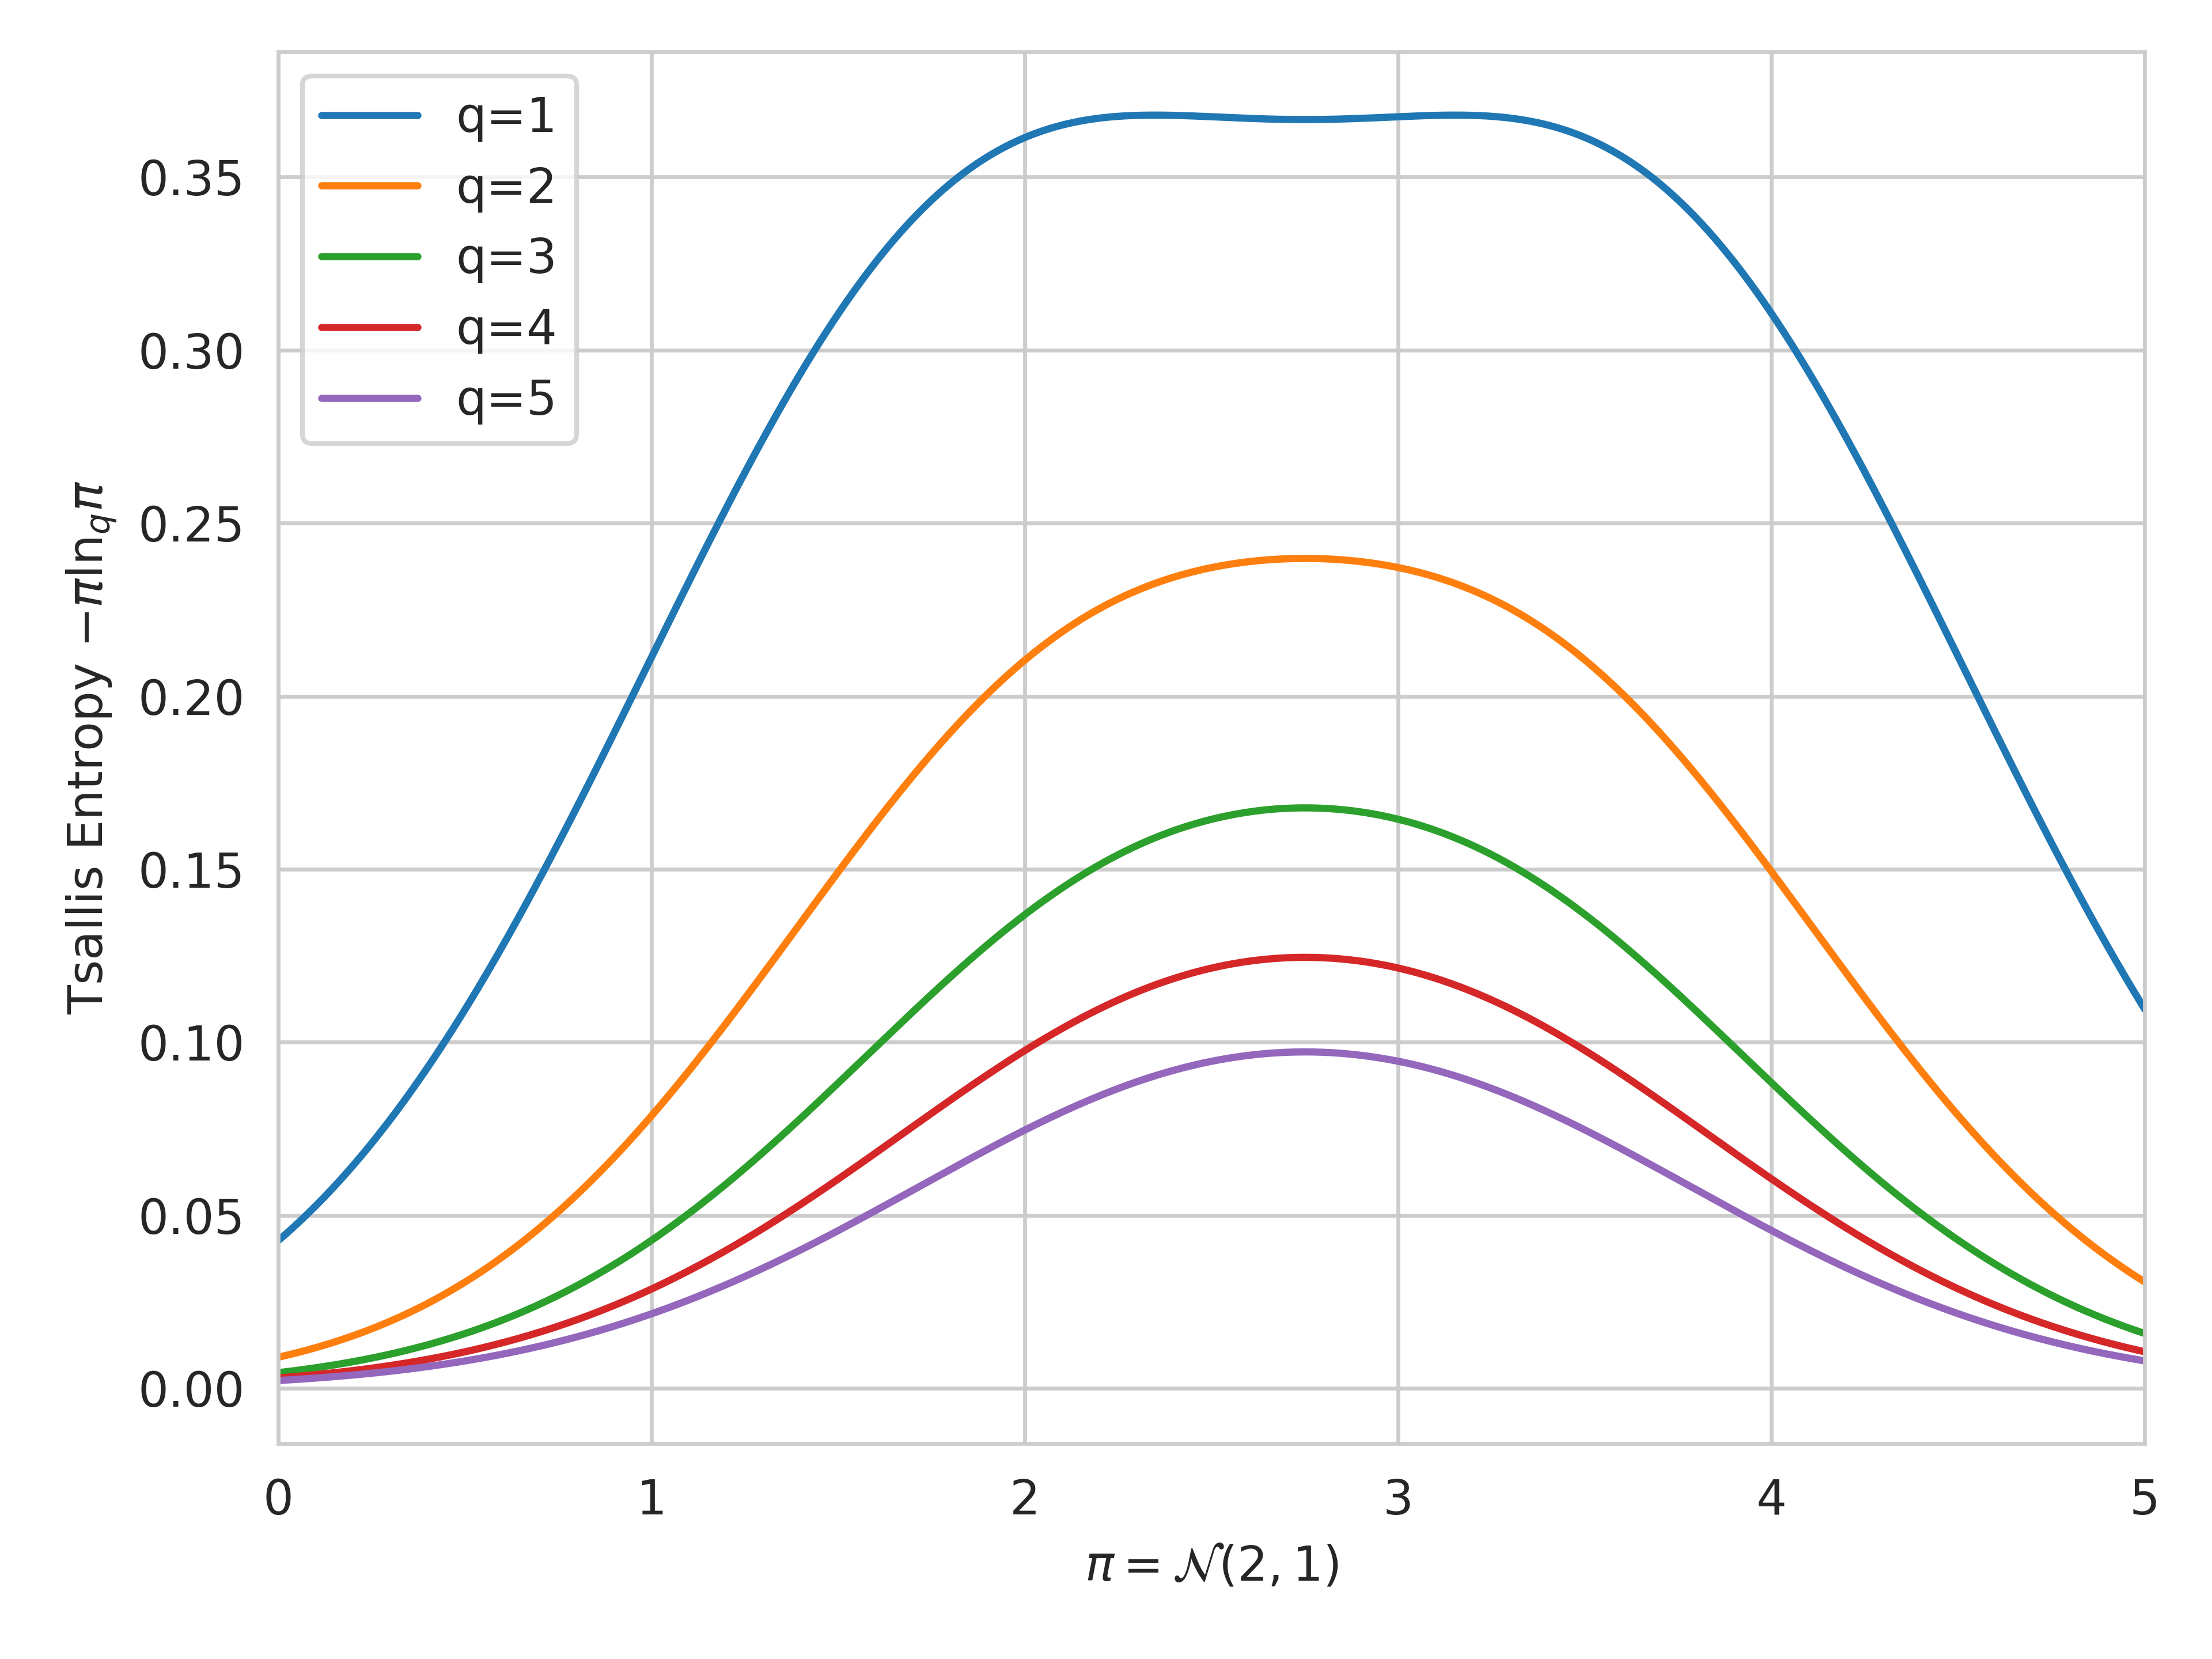
\includegraphics[width=\textwidth]{img/tsallis_entropy.png}
%         \label{fig:y equals x}
%     \end{subfigure}
%     \hfill
%     \begin{subfigure}[b]{0.49\textwidth}
%         \centering
%         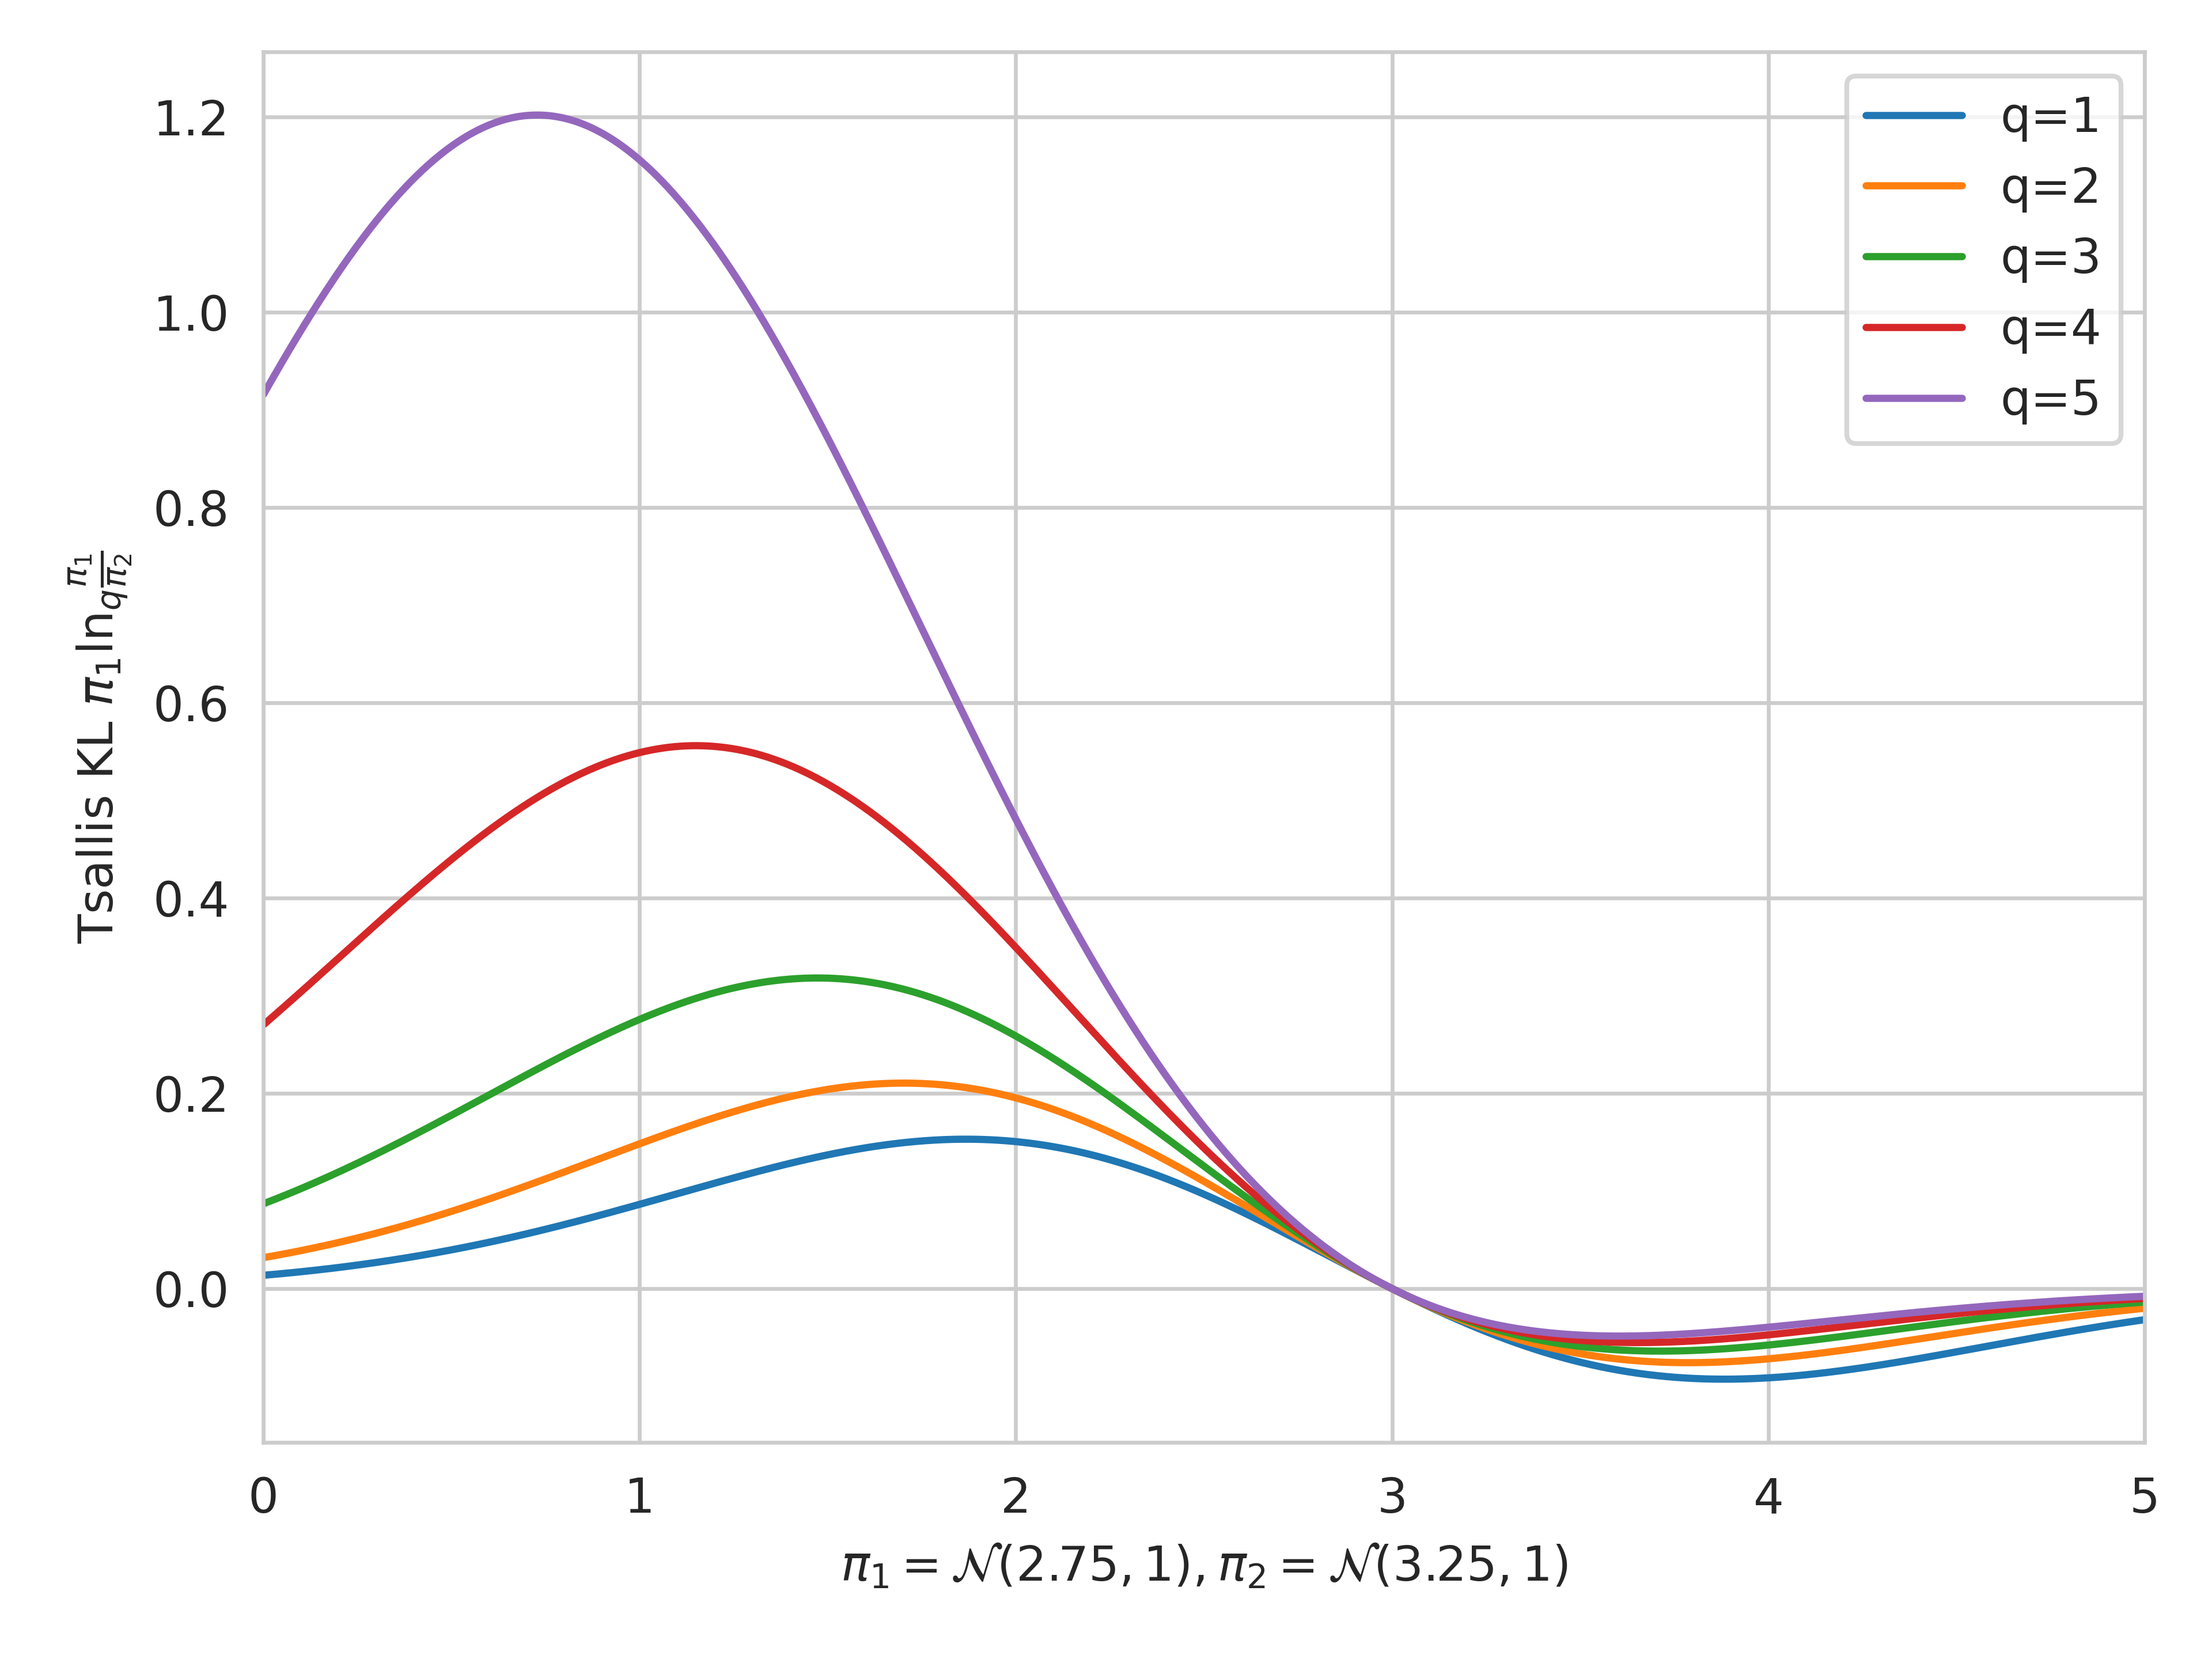
\includegraphics[width=\textwidth]{img/tsallis_kl.png}
%         \label{fig:three sin x}
%     \end{subfigure}
%     \caption{Estimation of policy ratio $\frac{\pi_{k+1}}{\pi_k}$ during learning of Munchausen DQN on \texttt{CartPole-v1} and \texttt{LunarLander-v2}.
%     Notice the $y$-axis is at the magnitude of $10^{35}$.
%     }
%     \label{fig:mdqn_policy_ratio}
% \end{figure}


Very recently \citet{zhu2023generalized} proposed in RL to exploit Tsallis KL divergence which generalizes Tsallis entropy.  
They proved that the regularized optimal policy takes a similar form to the optimal KL-regularized policy:
% Recall that, this definition is different from the statistical physics definition \citep{Furuichi2004-fundamentals-qKL}:
\begin{align}
    \begin{split}
        \qKLany{\pi(\cdot|s)}{\mu(\cdot|s)} = \sum_a \pi(a|s) \ln_{q} \frac{\pi(a|s)}{\mu(a|s)}, \quad \pi(a|s) = \mu(a|s) \exp_q\AdaBracket{\frac{Q_{\pi}(s,a)}{\tau} - \psi\AdaBracket{\frac{Q_{\pi}(s,a)}{\tau}} }.
    \end{split}
    \label{eq:tkl_policy}
\end{align}
We can also resort to Taylor's expansion and renormalization to obtain approximate policies, hence the policy can be written as $\pi(a|s)\propto \mu(a|s)\exp_q\AdaBracket{\frac{Q_{\pi}(s,a)}{\tau}}$.
It is worth noting that unlike the KL divergence, the Tsallis KL divergence cannot be decomposed as $\ln_q\!\frac{\pi(a|s)}{\mu(a|s)} \neq \ln_q \pi(a|s) - \ln_q \mu(a|s)$.
% \eq{\ref{eq:tkl_policy}} is important to our application of offline RL where we show the in-sample softmax becomes in-sample sparsemax.



\begin{figure}[t]
    \centering
    \begin{subfigure}[b]{0.245\textwidth}
        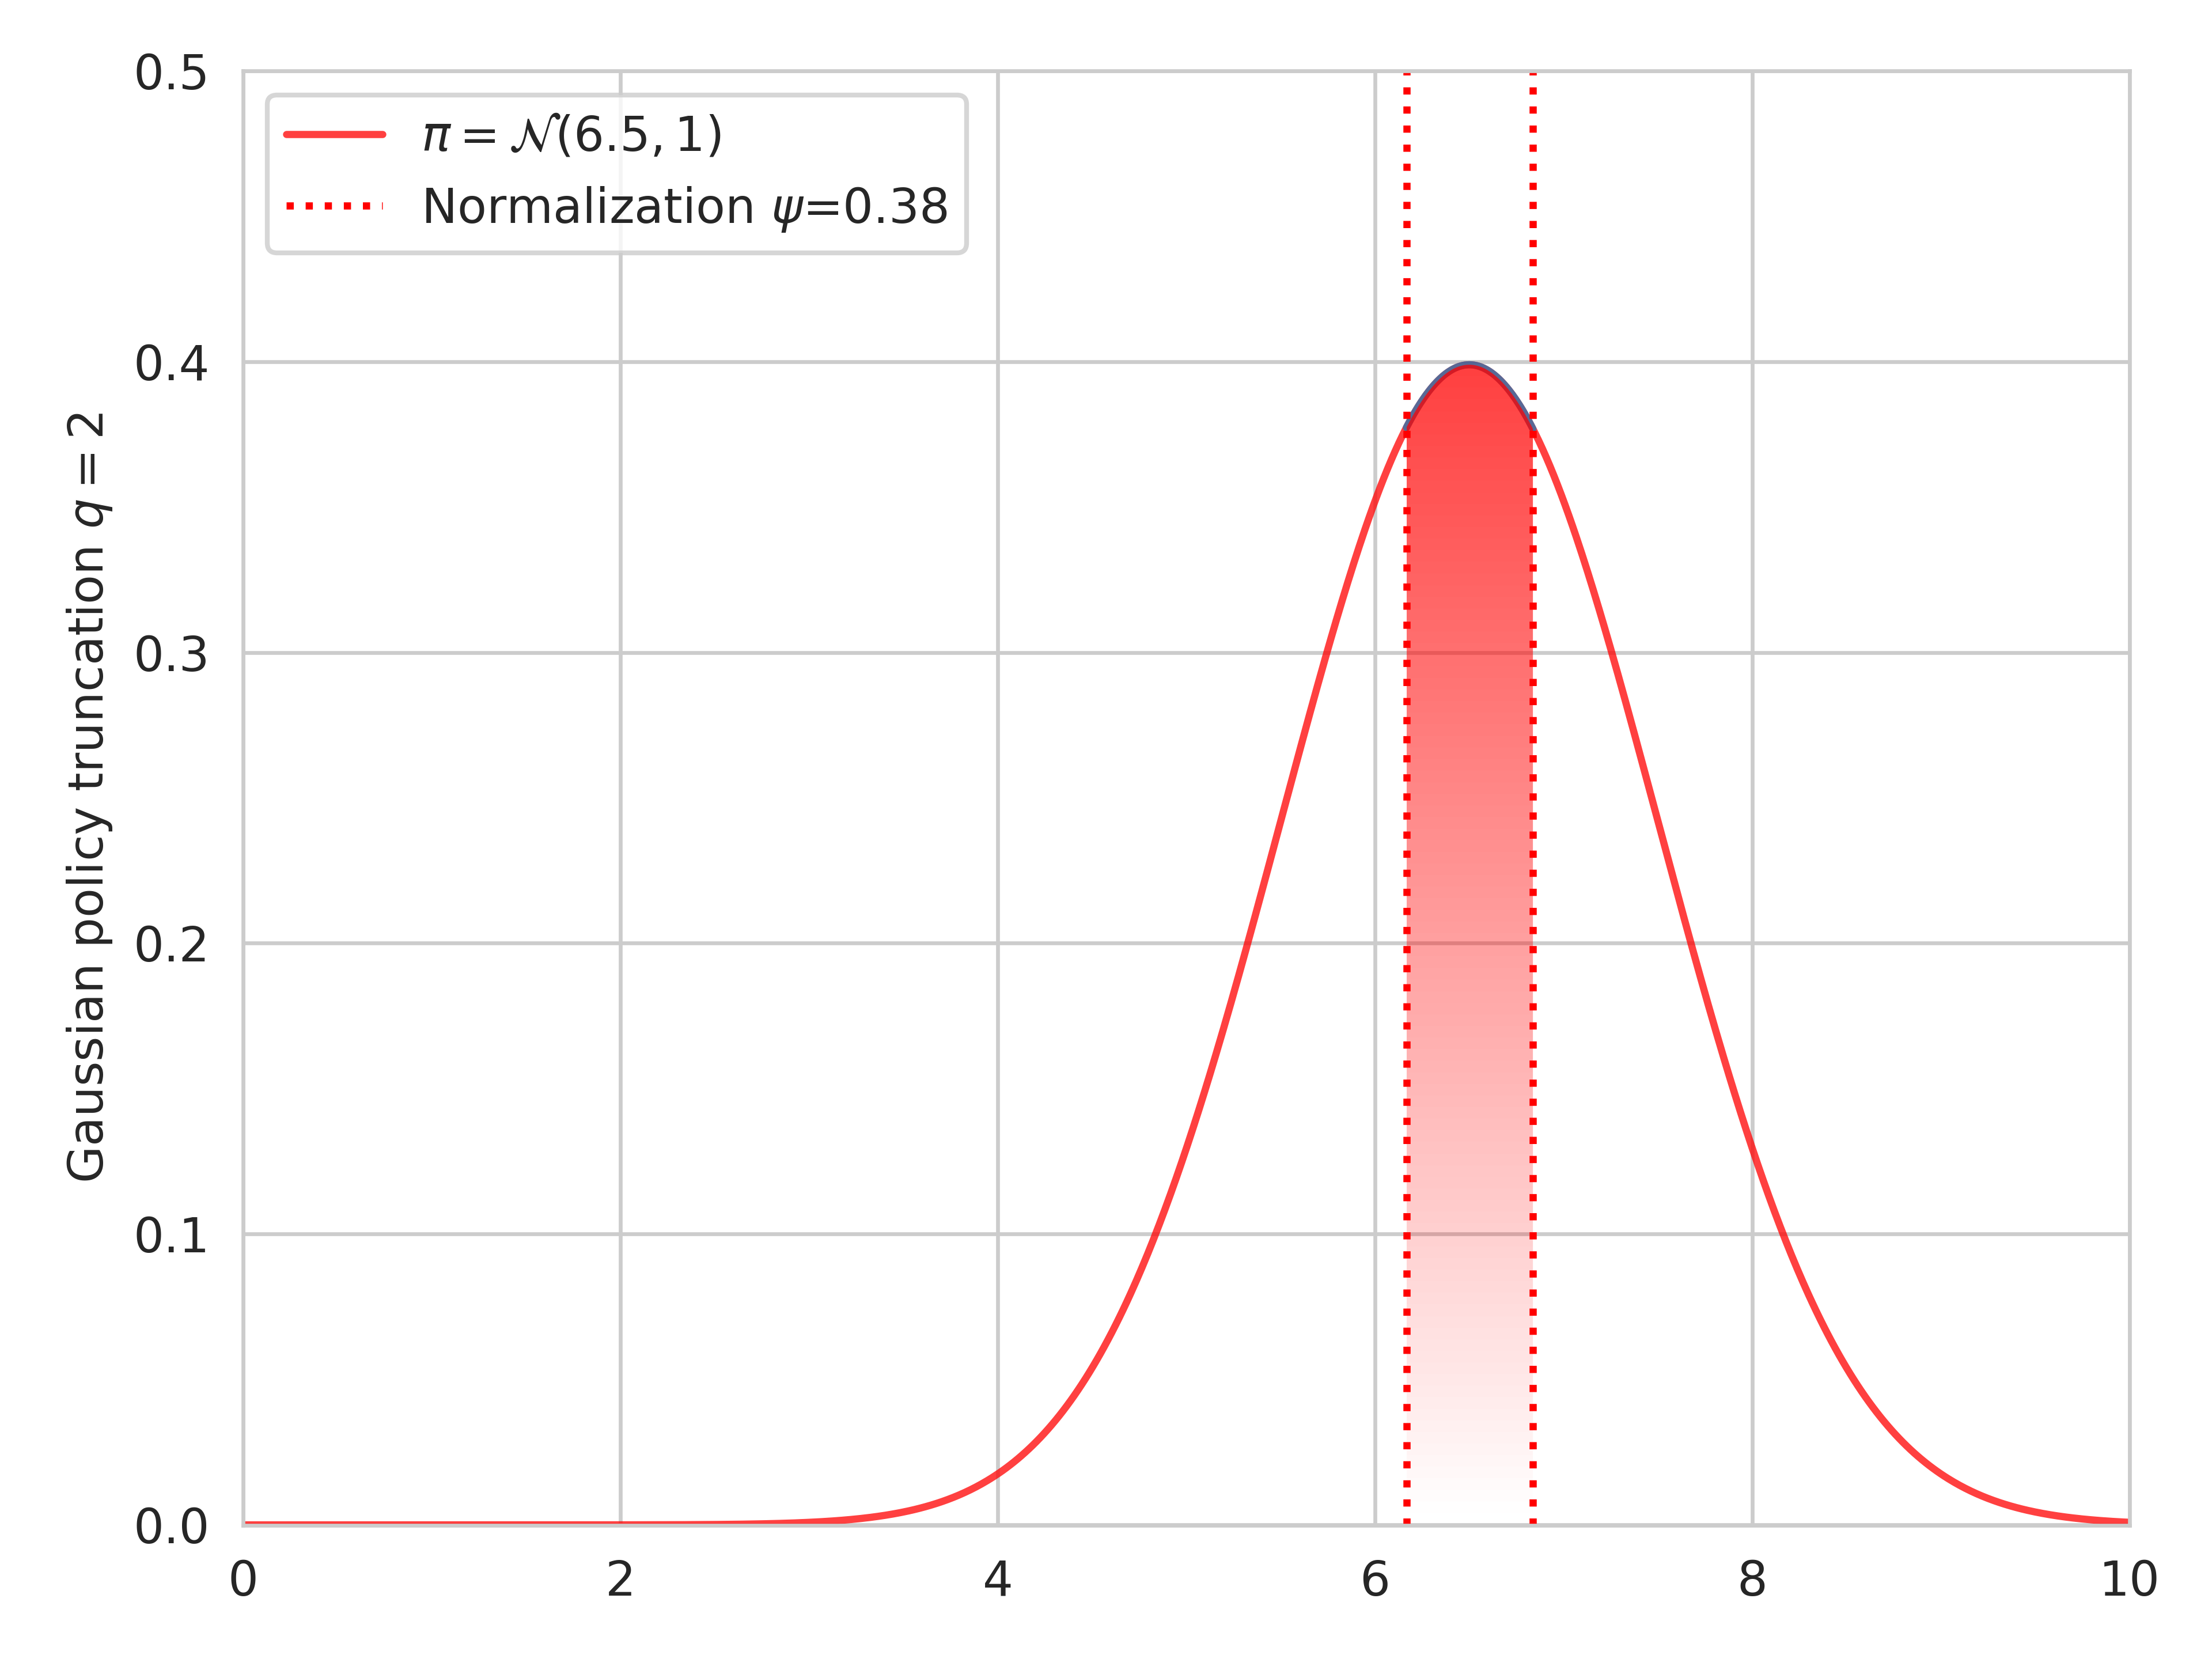
\includegraphics[width=\textwidth]{img/q2_Gaussian_sparsemax.png}
    \end{subfigure}
    \begin{subfigure}[b]{0.245\textwidth}
        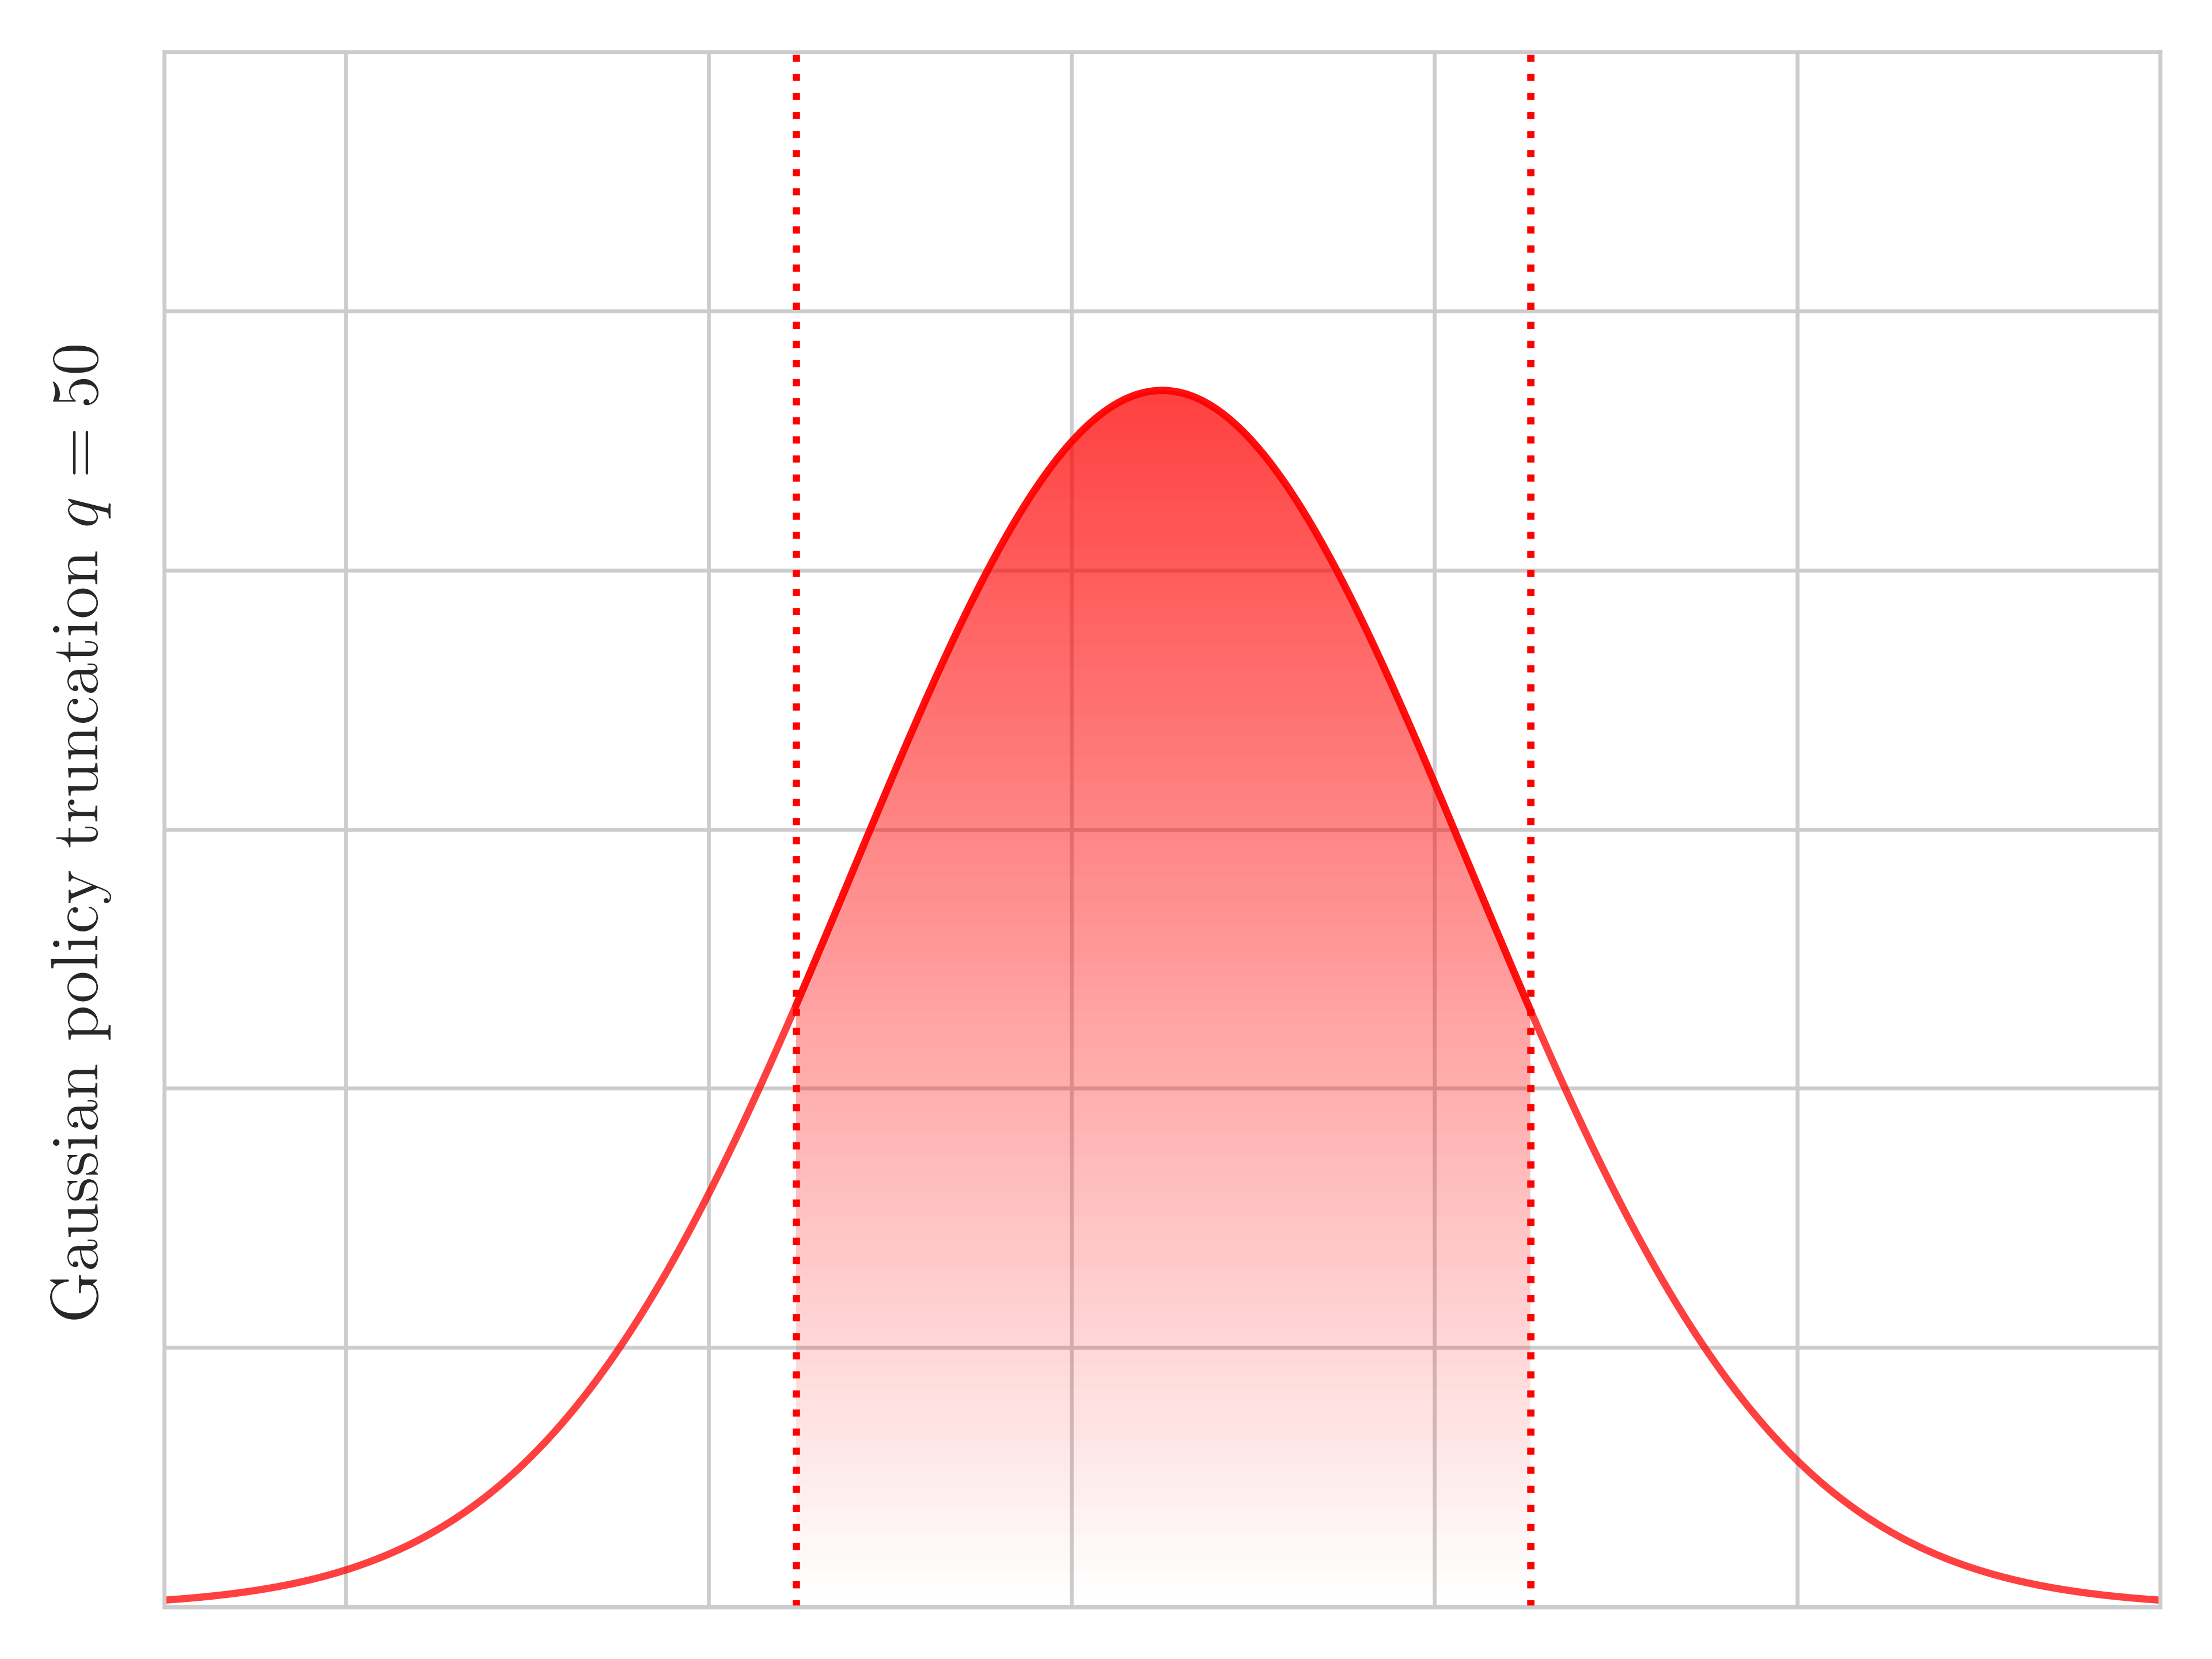
\includegraphics[width=\textwidth]{img/q50_scaled_Gaussian_sparsemax.png}
    \end{subfigure}
    \begin{subfigure}[b]{0.245\textwidth}
        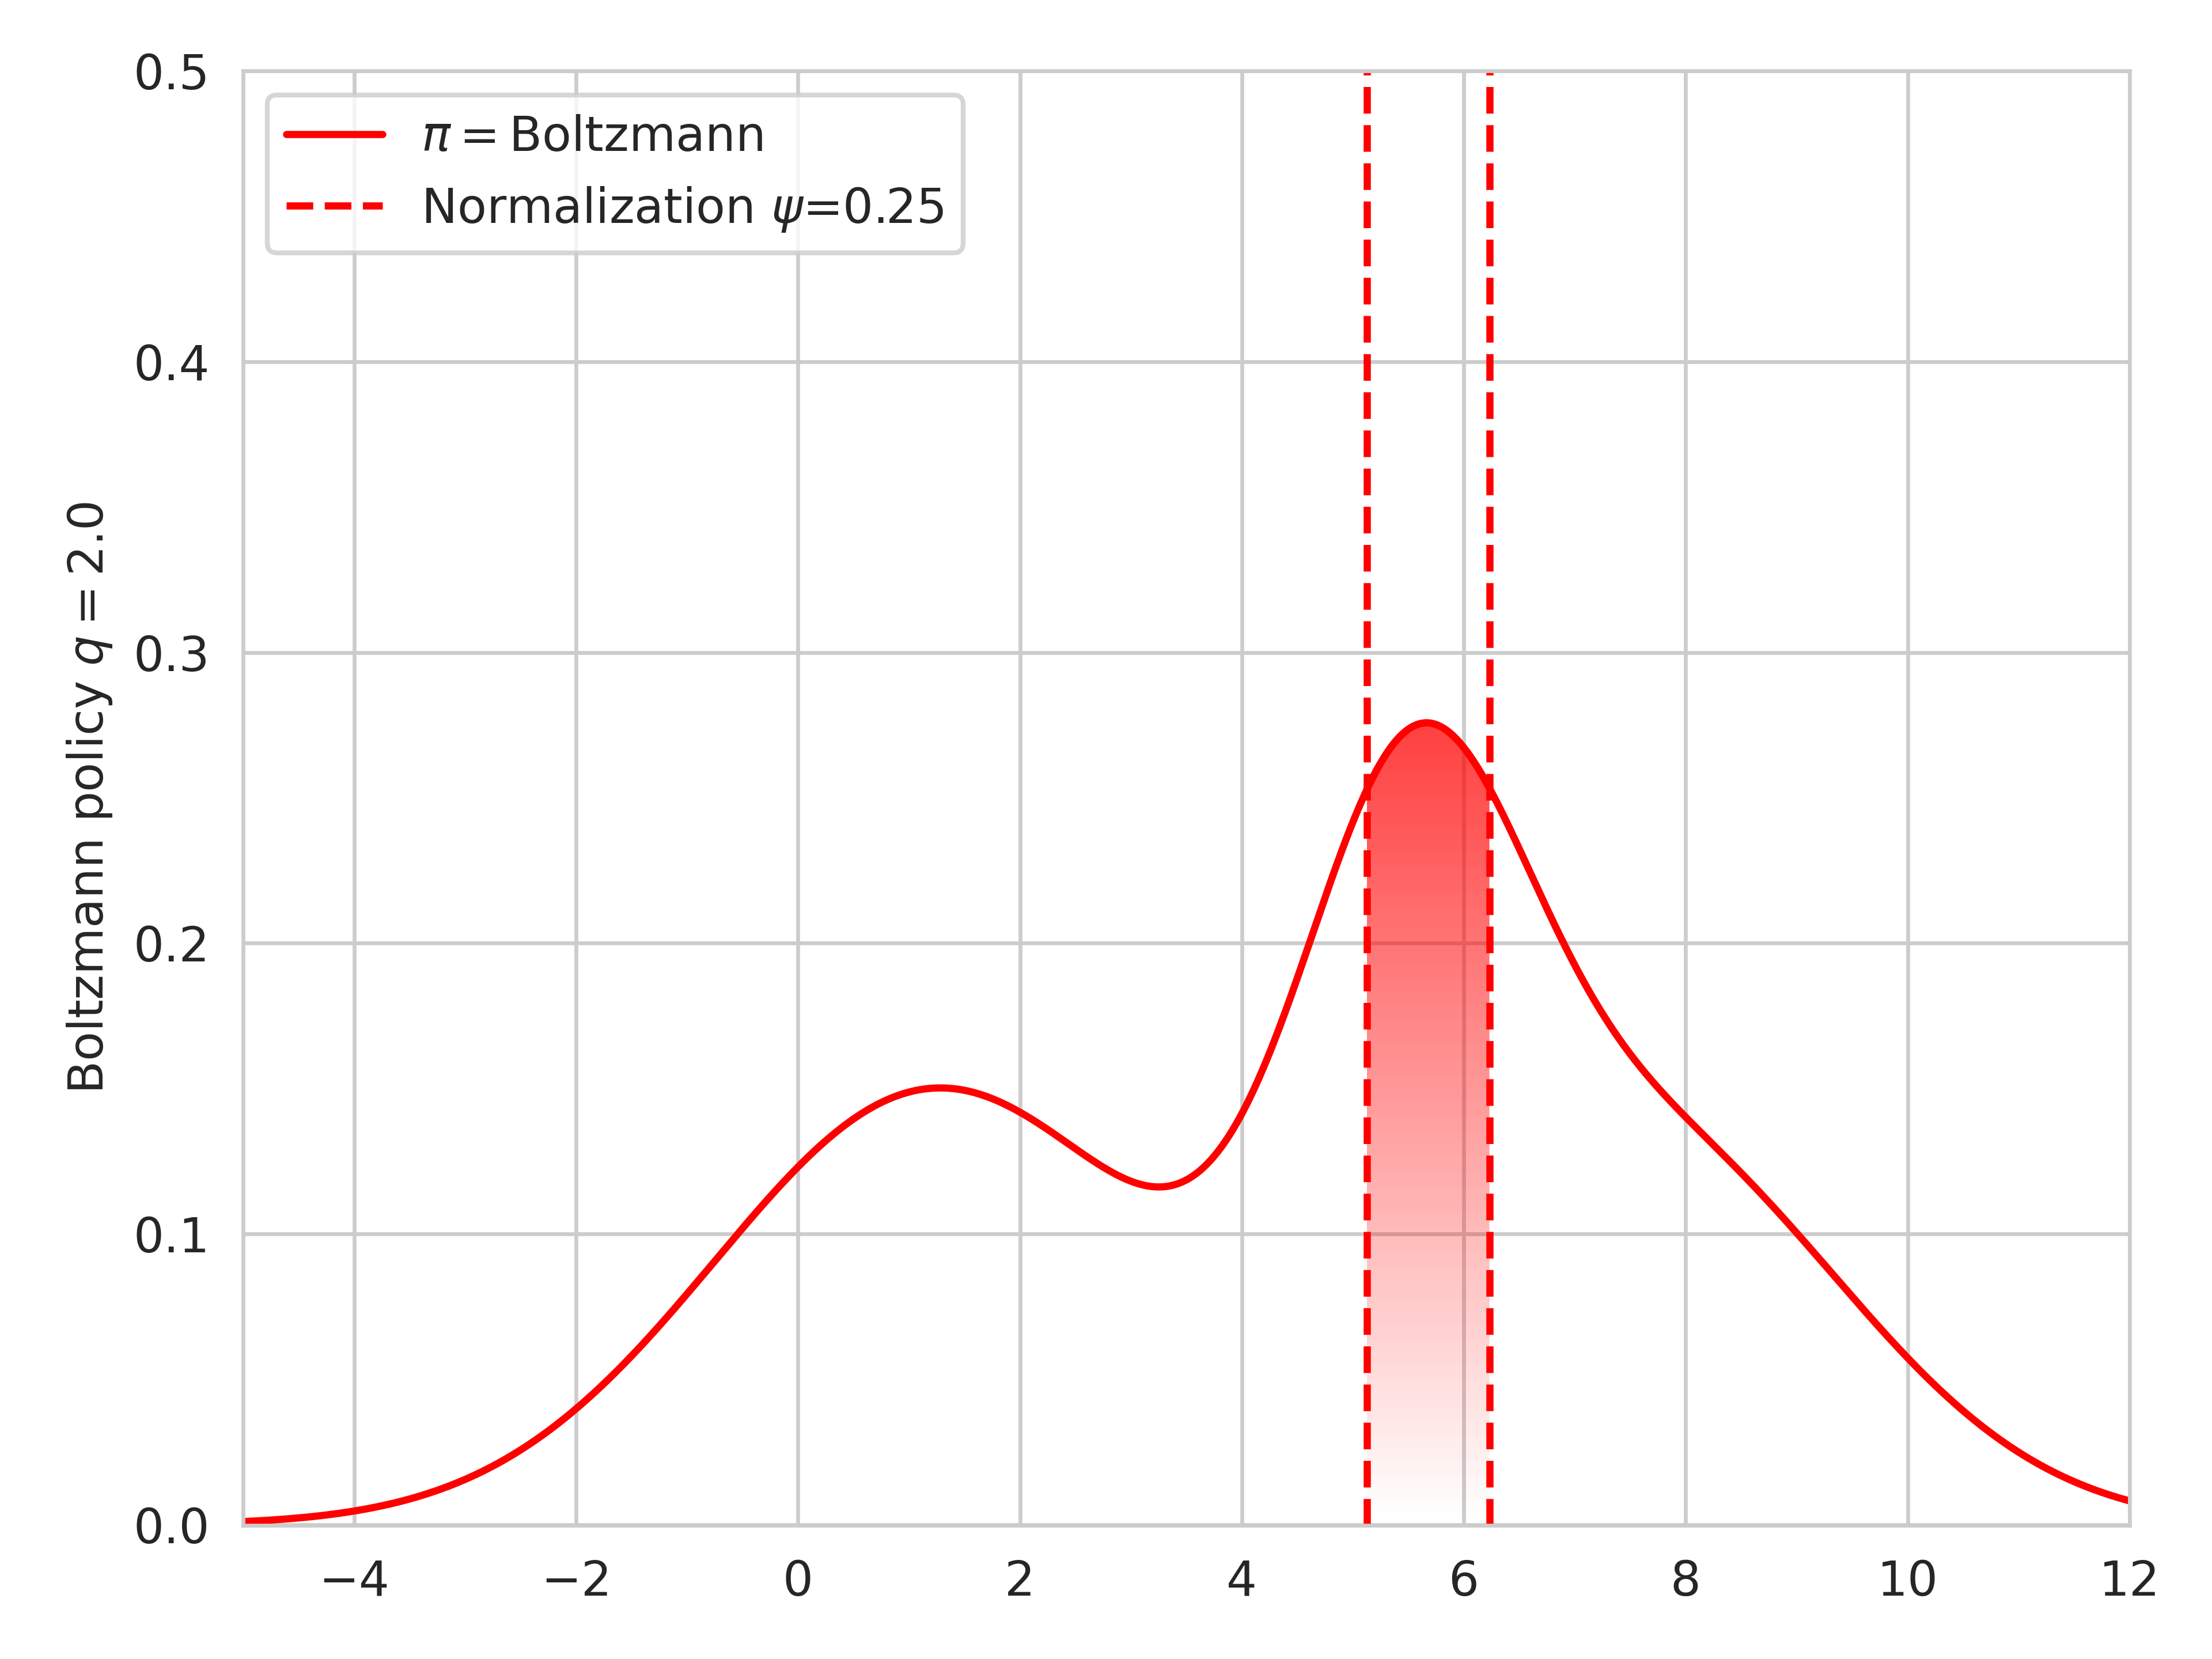
\includegraphics[width=\textwidth]{img/q2.0_Boltzmann_sparsemax.png}
    \end{subfigure}
    \begin{subfigure}[b]{0.245\textwidth}
        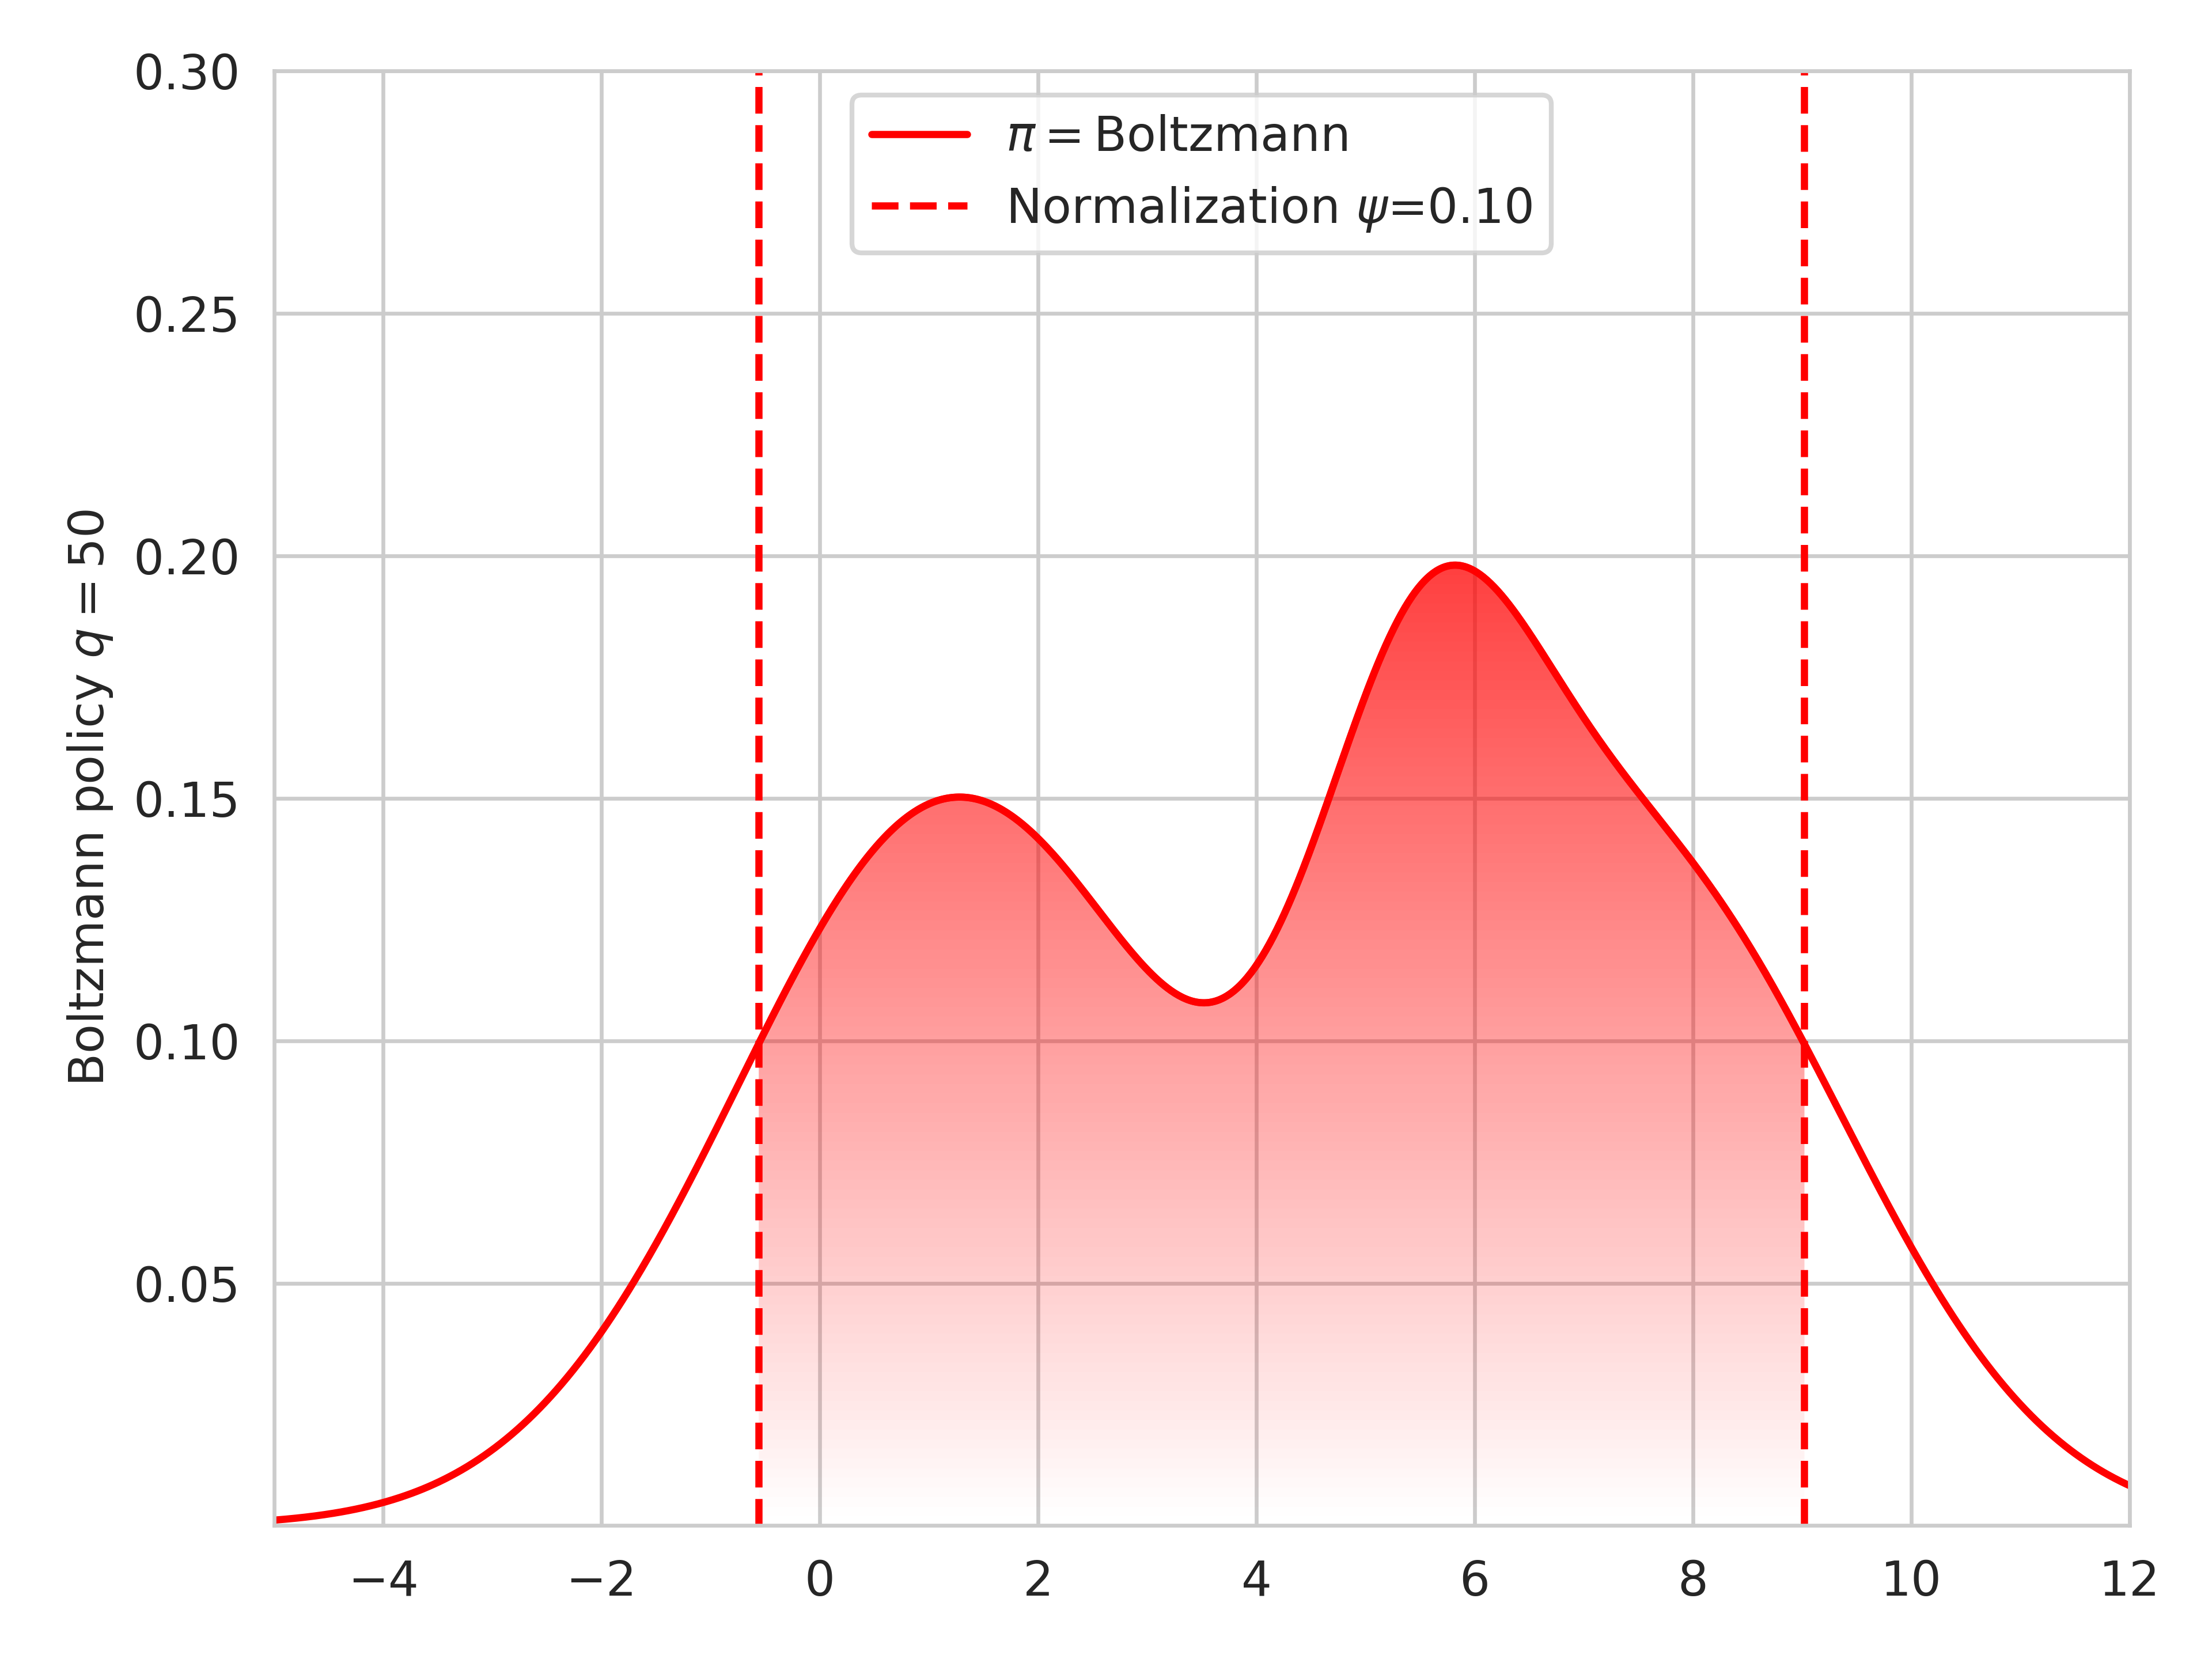
\includegraphics[width=\textwidth]{img/q50_Boltzmann_sparsemax.png}
    \end{subfigure}
    \caption{
        The sparsemax operator acting upon Gaussian and Boltzmann policies for $q=2$ and $q=50$ by truncating actions with values lower than $\psi$. 
    As $q\rightarrow \infty$ the policy tends toward uniform distribution.
    We assume the The dataset is generated by Tsallis policies such that the actions absent from the offline dataset are those being truncated.
    }
    \label{fig:q_truncation}
\end{figure}




\subsection{Offline Reinforcement Learning}

We consider the problem of offline RL, where the agent cannot interact with the environment and instead learn from a fixed dataset $\mathcal{D} = \{(s,a,r,s')_{1:N}\}$ collected by some unknown behavior policy $\datasetPolicy$.
The dataset $\mathcal{D}$ typically contains only a small subset of the $\mathcal{S}\times \mathcal{A}$ space.
Standard off-policy algorithms are known to suffer from the extrapolation error referring to the function approximator erroneously estimate action values for those out-of-distribution (OOD) actions not present in the dataset.
Extrapolation error can happen as a result of e.g. the smoothness of neural networks when the update is around some low sample region \cite{Gulcehre2021-regularizedBehavior}.
In the policy improvement step, the unrealistic high values of the OOD actions lead to target values that are further in favor of sampling OOD actions, causing a vicious loop. 

It is worth noting that unlike for online RL, where the OOD actions can lead to sampling more around the low sample region and eventually correction of the values, in offline RL this is impossible.
Instead, many of the existing works propose to force the learned policy to be close to the behavior policy \cite{Dadashi2021-pseudoMetricOffline,Fujimoto2019-InSampleMax,Fujimoto2021-minimalist,Nair2021-awac}.
This is often achieved by adding a regularizer in the policy update penalizing deviating from the behavior policy \cite{Ghasemipour2021-EMaQ,Kumar2019-BootstrapErrorQlearningMMD,Jaques2020-OfflineDialog,Wu2020-BehaviorRegularizedAC}, e.g. by incorporating KL divergence $\max_{\pi}\expectation{s\sim\mathcal{D}}{\expectation{a\sim\pi(\cdot|s)}{Q(s,a)} - \tau\KLany{\pi(\cdot|s)}{\datasetPolicy(\cdot|s)}}$.
The critic is typically updated by minimizing the loss $\mathbb{E}_{(s,a,s')\sim \mathcal{D}}\expectation{a\sim\pi(\cdot|s)}{\AdaBracket{ r(s,a) + \gamma Q(s',a') - Q(s,a)}^2}$.
The regularization leads to the policy form $\pi(a|s)\propto\datasetPolicy(a|s)\exp\AdaBracket{\tau^{-1}Q_{\pi}(s,a)}$ where the learned policy must have the same support of the behavior policy.
This idea is shared by the \emph{in-sample} methods that enforce the support of the learned policy to be within the behavior policy $\pi \preceq \datasetPolicy$ \cite{Fujimoto2019-InSampleMax,Kostrikov2022-implicitQlearning,Xiao2023-InSampleSoftmax}, which is achieved by only updating for the actions in the dataset.



\section{Method}

\subsection{In-Sample Softmax for Offline RL}


To alleviate the OOD error, \citet{Fujimoto2019-InSampleMax} proposed the in-sample Bellman optimality equation to update only for actions present in the dataset:
\begin{align}
    \datasetOptimalQ(s,a) = r(s,a) + \gamma \expectation{s'\sim P(\cdot | s,a)}{\max_{a': \datasetPolicy(a'|s') > 0} \datasetOptimalQ(s',a')}.
    \label{eq:hardmax_offline}
\end{align}
Later, \citet{Xiao2023-InSampleSoftmax} proposed in-sample softmax to better estimate the policy inside the bracket since in the continuous case the hard max operator might be difficult to solve for.
By regularizing with the Shannon entropy $\tau \entropy$ and imposing the dataset support constraint, the in-sample softmax Bellman optimality equation has the following evaluation step:
% \begin{align}
%     \datasetOptimalQ(s,a) = r(s,a) +  \gamma \expectation{s'\sim P(\cdot | s,a)}{ \sum_{a': \datasetPolicy(a'|s') > 0} \!\!\!\!\! \pi(a'|s') \AdaBracket{\datasetOptimalQ(s',a') - \tau\entropy(\cdot|s')}}.
%     \label{eq:insample_softmax}
% \end{align}
% By choosing the maximizer policy the above equation takes the form:
\begin{align}
    \datasetOptimalQ (s,a) = r(s,a) +  \gamma \expectation{s'\sim P(\cdot | s,a)}{\tau \ln \!\!\!\!\!\sum_{a': \datasetPolicy(a'|s') > 0} \!\!\!\!\! \exp\AdaBracket{\tau^{-1} \datasetOptimalQ(s',a')}}.
\end{align}
As the dataset support constraint poses a challenge to implementation, \citet{Xiao2023-InSampleSoftmax} proposed to transform the summation into an expectation to avoid directly computing the constraint: 
\begin{align}
    \begin{split}
    \sum_{a': \datasetPolicy(a'|s') > 0} \!\!\!\!\!\!\exp\AdaBracket{\tau^{-1}\datasetOptimalQ (s',a')} &= \!\!\!\!\!\!\sum_{a': \datasetPolicy(a'|s') > 0} \frac{\datasetPolicy(a'|s')}{\datasetPolicy(a'|s')} \exp\AdaBracket{\tau^{-1}\datasetOptimalQ (s',a')} \\
    &= \expectation{a'\sim\datasetPolicy(\cdot | s')}{\exp\AdaBracket{\tau^{-1}\datasetOptimalQ (s',a') - \ln\datasetPolicy(a'|s')}}.
    \end{split}
\end{align}
The expectation can be approximated by Monte-Carlo sampling actions from the dataset.
Since the term $\exp\AdaBracket{\tau^{-1}\datasetOptimalQ (s',a')}$ appears also in the regularized softmax policy, in-sample softmax updates the policy towards 
\begin{align}
    \pi_{t+1,\datasetPolicy} \propto  \datasetPolicy(a|s) \exp\AdaBracket{\frac{Q_{t, \datasetPolicy}(s,a)}{\tau} - \ln\hat{\pi}_{\mathcal{D}}(a|s)},
    \label{eq:inac_policy}
\end{align}
where $\hat{\pi}_{\mathcal{D}}$ inside the exponential function is learned to imitate the behavior policy to avoid $\pi_{\mathcal{D}} = 0$ leading to an unbounded log-policy.

The benefits of the in-sample softmax can be interpreted as (1) softmax is easier to compute than hard max in the continuous action setting; 
(2) the in-sample softmax policy \eq{\ref{eq:inac_policy}} can be seen as a KL-regularized policy and hence the dataset support constraint is satisfied.
In fact, the support of $ \pi_{\datasetPolicy, k+1}$ should be exactly the same as $\datasetPolicy$ since $\exp(\frac{\cdot}{\tau}) > 0$ as long as $\tau \neq \infty$.
We now explain why \eq{\ref{eq:inac_policy}} can be regarded as a KL-regularized policy: it can be decomposed into two terms:
the first term $\datasetPolicy(a|s) \exp\AdaBracket{\frac{Q_{t, \datasetPolicy}(s,a)}{\tau} }$ acts as a KL-regularized policy with respect to the behavior policy; 
the second term $\exp\AdaBracket{-\ln\hat{\pi}_{\mathcal{D}}(a|s)}$ can be seen as induced by another regularization $-\sum_{a}{\pi(a|s)}{\ln{\hat{\pi}_{\mathcal{D}}(a|s)}}$, which is the cross entropy between the in-sample softmax policy and the (learned) behavior policy.

However, the fact that the softmax policies always have full support indicates there is a persistent gap to \eq{\ref{eq:hardmax_offline}}.
Since we want to improve upon the behavior policy, it is expected that action candidates should gradually narrow down to the maximizer.
Furthermore, since \eq{\ref{eq:inac_policy}} is only implicitly regularizing the policy and no explicit KL regularization for the value estimation \cite{Wu2020-BehaviorRegularizedAC}, there is no guarantee that the learned policy should be close to the behavior policy.





\subsection{In-Sample Tsallis Regularization}

We propose to replace the Shannon entropy in in-sample softmax to the Tsallis entropy.
The seemingly simple replacement, however, leads to drastically different behavior of the policy.
Indeed, since we can control the truncation effect of the Tsallis regularized policies, we have the support of $\pi^{\text{Tsallis}}_{\datasetPolicy, k+1} \preceq \datasetPolicy$, i.e. the support of the learned policy is either equal or within the dataset support.

Furthermore, Tsallis policies provide an means to formulate the common assumption that actions not present in the dataset are with low probability of being selected \cite{Kostrikov2021-fisherCriticReg}.
If we assume the behavior policy is also a Tsallis policy, then the support constraint $a:\datasetPolicy(a|s)>0$ can be naturally replaced to the truncation criterion $a\in K(s)$; i.e.,
\begin{align}
    \datasetPolicy(a|s) \propto \exp_q\AdaBracket{\frac{Q_{\datasetPolicy}(s,a)}{\tau_\mathcal{D}}},  \quad \sum_{a\in K_\mathcal{D}(s)} \pi_\mathcal{D}(a|s)= 1,
\end{align}
where $\tau_\mathcal{D}$ is an unknown coefficient and $K_\mathcal{D}(s)$ denotes the set of actions present in the dataset.
% Now let us inspect the Bellman equation for the behavior policy:
% \begin{align}
%     \begin{split}
%     Q_{\datasetPolicy}(s,a) &= r(s,a) +  \gamma \expectation{s'\sim P(\cdot | s,a)}{ \sum_{a'} \datasetPolicy(a'|s') \AdaBracket{Q_{\datasetPolicy}(s',a') - \tau_{\mathcal{D}} S_2(\datasetPolicy)(\cdot|s')}}. \\ 
%     &= r(s,a) +  \gamma \expectation{s'\sim P(\cdot | s,a)}{ \tau_{\mathcal{D}} \AdaBracket{ \sum_{a' \in K_{\mathcal{D}}(s')} \AdaBracket{\frac{Q_{\datasetPolicy}(s',a')}{\tau_{\mathcal{D}}}}^2 - \psi \AdaBracket{\frac{Q_{\datasetPolicy}(s', \cdot)}{\tau_{\mathcal{D}}}}^2 + 1 }}\\
%     &= r(s,a) +  \gamma \expectation{s'\sim P(\cdot | s,a)}{ \tau_{\mathcal{D}} \AdaBracket{ \sum_{a': \datasetPolicy(a'|s') > 0} \AdaBracket{\frac{Q_{\datasetPolicy}(s',a')}{\tau_{\mathcal{D}}}}^2 - \psi \AdaBracket{\frac{Q_{\datasetPolicy}(s', \cdot)}{\tau_{\mathcal{D}}}}^2 + 1 }}.
%     \label{eq:insample_sparsemax}
%     \end{split}
% \end{align}
% Here, $\max_{\pi \in \Delta(\mathcal{A})}\pi(a|s)Q(s,a) + \tau S_2(\pi(\cdot|s)) $ attains its maximum at $V(s) = \tau \sum_{a \in K(s)}\AdaBracket{ \frac{Q(s,a)}{\tau} }^2 - \psi\AdaBracket{\frac{Q(s, \cdot)}{\tau}}^2 + \tau$ \cite{Lee2018-TsallisRAL,Martins16-sparsemax}.
% It is also possible to assume that $\datasetPolicy(a|s) = \exp_q\AdaBracket{\frac{Q_{\datasetPolicy}(s,a)}{\tau_\mathcal{D}} - \tilde{\psi}\AdaBracket{\frac{Q_{\datasetPolicy}(s, \cdot)}{\tau_\mathcal{D}}}}$ for general $q>2$, though in these cases the policy does not have a closed-form expression we have to resort to approximation.
Under the Tsallis behavior policy assumption, the dataset support constraint $a: \datasetPolicy(a|s) > 0$ coincides with the condition $a \in K_{\mathcal{D}}(s)$.
Revisiting the in-sample hard-max Bellman equation \eq{\ref{eq:hardmax_offline}}:
\begin{align*}
    \datasetOptimalQ(s,a) = r(s,a) + \gamma \expectation{s'\sim P(\cdot | s,a)}{\max_{a'\in K_{\mathcal{D}}(s)} \datasetOptimalQ(s',a')}.
\end{align*}
However, the assumption of the Tsallis behavior policy alone is not useful.
% Moreover, the assumption actually assumes a forward process of learning a set of allowable actions $K_\mathcal{D}(s)$ given $Q_{\datasetPolicy}(s,a), \forall s,a$;
%  and it naturally raises the possibility of \emph{backward Tsallis learning}: given the set of allowable actions $K_\mathcal{D}(s)$, learn an optimal policy that resembles $\datasetPolicy$ in the sense of $\pi_* \preceq \datasetPolicy$, i.e. putting probability mass only on the actions in $K_\mathcal{D}$.
The power of the assumption manifests when we use also Tsallis regularized policy learning:
% However, it should be noted that the learned policy no longer requires a thresholding function $\tilde{\psi}$ since the set of allowable actions $K_\mathcal{D}$ is given, hence no action need to be explicitly truncated.
% Specifically, we propose to modify the learned policy form as 
\begin{align}
    & \pi_{t+1, \datasetPolicy}(a|s) \propto \exp_q\AdaBracket{\frac{Q_{t, \datasetPolicy}(s,a)}{\tau}},  \quad \sum_{a\in K_{\mathcal{D}}(s)} \pi_{t+1, \datasetPolicy} (a|s) = 1.\\
    Q_{t+1, \datasetPolicy}(s,a) &= r(s,a) +  \gamma \expectation{s'\sim P(\cdot | s,a)}{ \sum_{a' \in K_{\mathcal{D}}(s)} \!\!\!\!\! \pi_{t+1}(a'|s') \AdaBracket{Q_{t, \datasetPolicy}(s',a') - \tau S_q(\pi_{t+1}(\cdot|s'))}}.
    \label{eq:proposal_policy}
\end{align}
The term inside the bracket is known as $q$-maximum \cite{Lee2020-generalTsallisRSS}.
Similar to the softmax operators \cite{asadi17a,azar2012dynamic}, $q$-maximum is an approximation to the maximum with degree controlled by $q$.

More importantly, the support constraint is naturally satisfied since 
the learned Tsallis policy learns a new set of allowable actions $K_{t, q}$ from $K_\mathcal{D}(s)$ depending on $q$ and iteration $t$.
The set satisfies the condition $K_{t, q} \preceq K_\mathcal{D}$:
 i.e. $|K_{t, q}| \leq |K_\mathcal{D}|$ and support constraint $\pi_t \preceq \datasetPolicy$.
 Let us take $q=2$ for example:
 \begin{align}
    \begin{split}
    &Q_{t+1, \datasetPolicy}(s,a) = r(s,a) +  \gamma \expectation{s'\sim P(\cdot | s,a)}{ \sum_{a' \in K_{\mathcal{D}}(s)} \!\!\!\!\! \pi_{t+1}(a'|s') \AdaBracket{Q_{t, \datasetPolicy}(s',a') - \tau S_2(\pi_{t+1}(\cdot|s'))}}\\
    &\qquad = r(s,a) + \gamma \expectation{s'\sim P(\cdot | s,a)}{ \tau\sum_{a' \in K_{\mathcal{D}}(s)} \!\! \AdaBracket{\frac{Q_{t, \datasetPolicy}(s',a')}{\tau}}^2 - \AdaBracket{ \psi\AdaBracket{\frac{Q_{t, \datasetPolicy}(s',a')}{\tau}} - 1 }^2 + \tau}\\
    &\qquad = r(s,a) + \gamma \expectation{s'\sim P(\cdot | s,a)}{ \tau\sum_{a' \in K_{t,q}(s)} \!\! \AdaBracket{\frac{Q_{t, \datasetPolicy}(s',a')}{\tau}}^2 - \AdaBracket{ \psi\AdaBracket{\frac{Q_{t, \datasetPolicy}(s',a')}{\tau}} - 1 }^2 + \tau}.
    \end{split}
    \label{eq:tsallis_backward_q2}
 \end{align}
 The second equation is because $\max_{\pi}\sum_{a\in\pi(\cdot|s)}\pi(a|s)Q(s,a) - \tau S_2(\pi(\cdot|s))$ attains its maximum at $\tau \sum_{a \in K(s)}\AdaBracket{ \frac{Q(s,a)}{\tau} }^2 - \psi\AdaBracket{\frac{Q(s, \cdot)}{\tau}}^2 + \tau$ \cite{Lee2018-TsallisRAL,Martins16-sparsemax}, and the last equation is due to $K_{t, q} \preceq K_\mathcal{D}$.
 \eq{\ref{eq:tsallis_backward_q2}} states that, one needs not to explicitly enforce the support constraint since it is automatically fulfilled by learning a new subset of allowable actions.
% That is, the backward Bellman optimality equation becomes:
% \begin{align}
%     \begin{split}
%         \datasetOptimalQ(s,a) &= r(s,a) +  \gamma \expectation{s'\sim P(\cdot | s,a)}{ \sum_{a' \in K_\mathcal{D}(s')} \pi_{*, \datasetPolicy}(a'|s') \AdaBracket{\datasetOptimalQ(s',a') - \tau S_2(\pi_{*, \datasetPolicy})(\cdot|s')}}. 
%     \end{split}
% \end{align}
% The term inside the expectation is now:
% \begin{align}
%     \begin{split}
%         & \sum_{a' \in K_\mathcal{D}(s')} \pi_{*, \datasetPolicy}(a'|s') \AdaBracket{\datasetOptimalQ(s',a') - \tau S_2(\pi_{*, \datasetPolicy})(\cdot|s')} \\ 
%          &= \sum_{a' \in K_\mathcal{D}(s')} \pi_{*, \datasetPolicy}(a'|s') \AdaBracket{ \datasetOptimalQ(s',a') + \frac{\tau}{2}(1 - \pi_{*, \datasetPolicy}(a'|s')) } \\
%          &= \sum_{a' \in K_\mathcal{D}(s')} \pi_{*, \datasetPolicy}(a'|s') \AdaBracket{ \datasetOptimalQ(s',a') - \frac{\tau}{2}\pi_{*, \datasetPolicy}(a'|s') } + \frac{\tau}{2} \\
%          &= \sum_{a' \in K_\mathcal{D}(s')} \frac{\AdaRectBracket{ \tau^{-1}Q_{t, \datasetPolicy}(s,a)}_+ }{\sum_{b\in K_\mathcal{D}(s')}\tau^{-1} Q_{t, \datasetPolicy}(s,b)}
%     \end{split}
% \end{align}

We now show that, if the Tsallis behavior policy assumption holds and we use Tsallis regularized policy learning, then the learned policy is guaranteed to stay close to the behavior policy in the sense that their KL divergence is uppper-bounded.
\begin{theorem}
    Suppose the dataset $\mathcal{D}$ is generated by a Tsallis behavior policy of entropic index $q$.
    Let $K_{t, q}(s) \preceq K_\mathcal{D}(s)$ denote the set of allowable actions at $t$-th iteration whose cardinality is smaller than $K_\mathcal{D}(s)$.
    Also let $\pi_{t}(a|s) \propto \exp_q\AdaBracket{\frac{Q_{t-1}(s,a)}{\tau}}$ denote the learned policy. 
    Then the KL divergence between $\pi_t$ and the behavior policy can be upper bounded:
\begin{align}
    \begin{split}
    &\KLany{\pi_t(\cdot|s)}{\datasetPolicy(\cdot|s)}  \leq  |K_{t,q}(s)|\! \AdaRectBracket{  { \pi_{t}^{q}(a|s) - \pi_{t}^{q-1} (a|s) } + \pi_t(a|s) - \frac{q-3}{q-1}  + \datasetPolicy^{q-2}(a|s) - \datasetPolicy^{q-1}(a|s)}.
\end{split}
\end{align}
\end{theorem}
The bound is suggestive.
For $q=1$ (the in-sample softmax case) the bound is not useful and simply states the KL divergence may be unbounded.
On the other hand, choosing any $q>1$ brings an upper bound of at most $4 |K_{t,q}(s)|$.
When  $q=2$, the in-sample sparsemax has KL divergence to the behavior policy bounded by $|K_{t, q}(s)|\AdaBracket{\pi_t(a|s) - \pi_\mathcal{D}(a|s) + 2}$.
However, it should be noted that there is a trade-off between the power of policies $\pi^{q}$ and the cardinality of $K_{t,q}(s)$: $K_{t,q}(s)$ tends to collect all actions when $q \rightarrow \infty$.
\begin{proof}
    We first prove the following lemma:
\begin{lemma}\label{lemma:log_qlog_diff}
    The difference between the standard logarithm and $q$-logarithm can be expressed by:
    \begin{align*}
        \ln x - \ln_q x = (q-1) \AdaRectBracket{\frac{d}{dq}\ln_q x - \ln x \ln_q x}.
    \end{align*}
\end{lemma}
\begin{proof}
    Let us begin with the right hand side 
    \begin{align*}
        &(q-1) \AdaRectBracket{\frac{d}{dq}\ln_q x - \ln x \ln_q x} = (q-1) \AdaRectBracket{\frac{d}{dq} \frac{x^{q-1} - 1}{q-1} -  \ln x \ln_q x}\\
        &= (q-1) \AdaRectBracket{ \frac{(x^{q-1} - 1)'(q-1) - (x^{q-1} - 1)(q-1)'}{(q-1)^2  } -  \ln x \ln_q x }\\
        &= (q-1) \AdaRectBracket{ \frac{(q-1) x^{q-1}\ln x - (x^{q-1} - 1)}{(q-1)^2  } -  \ln x \ln_q x }\\
        &= x^{q-1}\ln x - \ln_q x - (q-1)\ln x\ln_q x = \AdaBracket{(q-1)\ln_q x + 1} \ln x - \ln_q x - (q-1)\ln x\ln_q x\\
        &= \ln x - \ln_q x.
    \end{align*}
\end{proof}
With the lemma, we have the following theorem indicating the Tsallis backward learning  policies have bounded distance to the behavior policy:
    We decompose the KL divergence into three terms and apply Lemma \ref{lemma:log_qlog_diff}:
\begin{align}
    \begin{split}
        &\KLany{\pi_t(\cdot|s)}{\datasetPolicy(\cdot|s)} = \expectation{a\sim\pi_{t}(\cdot | s)}{\ln \pi_{t}(a|s) - \ln\datasetPolicy(a|s)} \\
        & = \expectation{a\sim\pi_{t}(\cdot | s)}{\underbrace{\ln \pi_{t}(a|s) - \ln_q\pi_{t}(a|s)}_{(1)} + \underbrace{\ln_q\pi_{t}(a|s) -  \ln_q\datasetPolicy(a|s)}_{(2)} + \underbrace{\ln_q\datasetPolicy(a|s) - \ln\datasetPolicy(a|s)}_{(3)} } .
    \end{split}
\end{align}
Let us now respectively bound the three terms:
\begin{align}
    \begin{split}
        (1): &\ln \pi_{t}(a|s) - \ln_q\pi_{t}(a|s) = (q-1) \AdaRectBracket{\frac{d}{dq}\ln_q \pi_t(a|s) - \ln_q\pi_t(a|s)\ln\pi_t(a|s)}\\
        % &= (q-1)\AdaRectBracket{\pi_t^{q-1}(a|s)\ln\pi_t(a|s) - \frac{\pi_{t}^{q-1}(a|s)-1}{(q-1)^2} - \ln_q\pi_t(a|s)\ln\pi_t(a|s)}\\
        &= \pi_{t}^{q-1}(a|s)\ln\pi_t(a|s) - \ln_q\pi_t(a|s) - (q-1)\ln_q\pi_t(a|s)\ln\pi_t(a|s)\\
        % &= (q-1)\pi_{t}^{q-1}(a|s)\ln\pi_t(a|s) - \AdaBracket{ \frac{Q_{t-1}(s,a)}{\tau} - \tilde{\psi}\AdaBracket{\frac{Q_{t-1}(s,\cdot)}{\tau}}}  + \ln\pi_t(a|s) \AdaBracket{ \frac{Q_{t-1}(s,a)}{\tau} - \tilde{\psi}\AdaBracket{\frac{Q_{t-1}(s,\cdot)}{\tau}}}
        & \leq \pi_{t}^{q-1}(a|s)\ln\pi_t(a|s) + \frac{1}{q-1} + \ln\pi_t (a|s)\\
        & \leq  \AdaBracket{ \pi_{t}^{q}(a|s) - \pi_{t}^{q-1} (a|s) } + \pi_t(a|s) - \frac{q-2}{q-1},
    \end{split}
\end{align}
where we leveraged $\ln x \leq x - 1$ and  $\ln_q\exp_q(x) = x$ both when $x>0$.
Considering the definition of $\pi_t(a|s) \propto \exp_q\AdaBracket{\frac{Q_{t-1}(s,a)}{\tau} - {\psi}\AdaBracket{\frac{Q_{t-1}(s,\cdot)}{\tau}}}$ and $\exp_q(x) = \AdaRectBracket{1 + (q-1)x}_{+}^{\frac{1}{q-1}}$, we must have  $\pi_t(a|s) > 0 \Leftrightarrow a\in K_{t-1,q}(s) \Leftrightarrow -\frac{1}{q-1} \leq \frac{Q_{t-1}(s,a)}{\tau} - {\psi}\AdaBracket{\frac{Q_{t-1}(s,\cdot)}{\tau}} \leq 0$. 
If $a \notin K_{t-1,q}(s)$, then $\ln\pi_t(a|s) = -\infty$ and the KL term is unbounded.
The same fact is exploited to yield an upper bound $\frac{1}{q-1}$  for (2).
We now work with (3):
\begin{align}
    \begin{split}
        (3): &\ln_q \datasetPolicy(a|s) - \ln\datasetPolicy(a|s) = -(q-1) \AdaRectBracket{\frac{d}{dq}\ln_q \datasetPolicy(a|s) - \ln_q\datasetPolicy(a|s)\ln\datasetPolicy(a|s)}\\
        % &= -\pi_{t}^{q-1}(a|s)\ln\pi_t(a|s) + \ln_q\pi_t(a|s) + (q-1)\ln_q\pi_t(a|s)\ln\pi_t(a|s)\\
        & \leq -\datasetPolicy^{q-1}(a|s)\ln\datasetPolicy(a|s)  \leq  -\datasetPolicy^{q-1}(a|s)\AdaBracket{1 - \frac{1}{\datasetPolicy(a|s)} } = \datasetPolicy^{q-2}(a|s) - \datasetPolicy^{q-1}(a|s).
    \end{split}
\end{align}
Putting all terms together, we arrive at the upper bound that 
\begin{align*}
    \KLany{\pi_t(\cdot|s)}{\datasetPolicy(\cdot|s)} &\leq \!\!\!\!\!\! \sum_{a\in K_{t,q}(s)}\!\!\!\!\! \pi_t(a|s)\AdaRectBracket{  { \pi_{t}^{q}(a|s) - \pi_{t}^{q-1} (a|s) } + \pi_t(a|s) - \frac{q-3}{q-1}  + \datasetPolicy^{q-2}(a|s) - \datasetPolicy^{q-1}(a|s)} \\
    &\leq K_{t,q}(s)\!\AdaRectBracket{  { \pi_{t}^{q}(a|s) - \pi_{t}^{q-1} (a|s) } + \pi_t(a|s) - \frac{q-3}{q-1}  + \datasetPolicy^{q-2}(a|s) - \datasetPolicy^{q-1}(a|s)}.
\end{align*}

\end{proof}

The assumption of Tsallis behavior policy is not restrictive.
If all actions present, then it corresponds to the case of $q=1$ where the policy has full support.
On the other hand, different levels of missingness can be simulated by both $q$ and $\tau$.

Another advantage of \eq{\ref{eq:proposal_policy}} is that for $q>1$, the policy is a variant of categorical distributions which is less susceptible to numerical issues than exponential functions \cite{Tsai2021-selfsupervisedRelativePredictiveCoding}.
Furthermore, \eq{\ref{eq:proposal_policy}} can switch between greedy policy and multimodal policy.
The former is achieved when all but one action have values lower than the threshold; while vice versa for the latter.


\textbf{In-sample Tsallis Policy Estimation}
Similar to \cite{Xiao2023-InSampleSoftmax}, we want to directly use the actions from the dataset to estimate our policy.
We do a similar step to \eq{\ref{eq:inac_policy}}:
\begin{align}
    \begin{split}
        &\pi_{t+1,\datasetPolicy} (a|s) \propto \exp_q \AdaBracket{\frac{1}{\tau} Q_{t, \datasetPolicy}(s,a)} = \datasetPolicy(a|s) \datasetPolicy(a|s)^{-1} \exp_q\AdaBracket{\frac{1}{\tau}Q_{t, \datasetPolicy}(s,a)} \\
        &= \datasetPolicy(a|s)  \exp_q{\AdaBracket{\ln_q{\frac{1}{\datasetPolicy(a|s)}}}} \exp_q\AdaBracket{\frac{1}{\tau}Q_{t, \datasetPolicy}(s,a)}\\
        &=  \datasetPolicy(a|s) {\AdaBracket{ \exp_q\AdaBracket{\frac{1}{\tau}Q_{t, \datasetPolicy}(s,a) + \ln_q\frac{1}{\datasetPolicy(a|s)}}^{q-1} - (q-1)^2 \frac{1}{\tau}Q_{t, \datasetPolicy}(s,a)  \ln_q{\frac{1}{\datasetPolicy(a|s)}} }^{\frac{1}{q-1}}}.
        \label{eq:tsallis_inac_policy_thoery}
    \end{split}
\end{align}
In the last step we made use of the relationship $\AdaBracket{\expq{x}\cdot \expq{y}}^{q-1} = \expq{\AdaBracket{x+y}}^{q-1} + (q-1)^2 xy$ \cite{Yamano2004-properties-qlogexp}.

\begin{remark}
    Tsallis entropy regularization has not been popular since its proposal in RL \cite{Lee2018-TsallisRAL}.
    One of the main reasons is the sparsemax policies are not suitable for online RL since the exploration is handicapped resulted from the action truncation.
    However, in offline RL this drawback vanishes, and theoretically it allows for bounding the distance to the behavior policy, guaranteeing less OOD actions.
\end{remark}


\section{Implementation}

Let $\theta, \phi, \omega$ denote the parametrization of networks for $Q$, $\pi_{\datasetPolicy}, \datasetPolicy$, respectively.
In-sample softmax updates the policy towards 
\begin{align}
    \pi_{\datasetPolicy, Q_{\theta}}(a|s) = \datasetPolicy(a|s)\exp\AdaBracket{\frac{Q_{\theta}(s,a) - Z(s)}{\tau} - \ln \pi_{\omega}(a|s)},
    \label{eq:insample_policy}
\end{align}
where $Z(s)$ denotes the normalization constant and is necessary since the policy is updated by minimizing KL divergence:
\begin{align*}
    &\KLany{\pi_{\datasetPolicy, Q_{\theta}}(\cdot|s)}{\pi_{\phi}(\cdot | s)} = \expectation{a \sim \pi_{\datasetPolicy, Q_{\theta}}(\cdot|s) }{\ln \pi_{\datasetPolicy, Q_{\theta}}(a|s) - \ln \pi_{\phi}(a | s)} \\
    &= \expectation{a \sim \datasetPolicy(\cdot|s)}{ - \exp\AdaBracket{\frac{Q_{\theta}(s,a) - Z(s)}{\tau} - \ln \pi_{\omega}(a|s)} \ln\pi_{\phi}(a|s) },
\end{align*} 
where the $\datasetPolicy$ term in $ \pi_{\datasetPolicy, Q_{\theta}}$ is absorbed into the expectation, so the KL divergence loss can be minimized by sampling actions from the offline dataset.

We follow the same setup here, but replacing every appearance of $\ln, \exp$ to their \qlog and $q$-exponential counterpart.
% In practice, computing the thresholding function $\psi$ requires sorting in the discrete control setting and it remains unclear how to accurately estimate it for the continuous control problems.
% We found it improves the performance by simply removing $\psi$ and renormalize the policy.
% In this case, thresholding can still be achieved by simply learning $Q_{\theta} \rightarrow 0$.
% That is, the learned policy form becomes $\pi_{t+1}(a|s) \propto \AdaRectBracket{Q_{\theta}(s,a)}_{+}$.
% In order to also sample actions from the dataset when updating the policy, we repeat the derivation in \eq{\ref{eq:insample_policy}} but for the sparsemax policy.
% % Let us define $q_{\theta}(s,a) := \frac{Q_{\datasetPolicy, k}(s,a)}{\tau} - \psi\AdaBracket{\frac{Q_{\datasetPolicy, k}(s,\cdot)}{\tau}}$ for convenience:
% \begin{align}
%     \begin{split}
%         \pi_{\datasetPolicy, k+1} (a|s) &= \datasetPolicy(a|s) \datasetPolicy(a|s)^{-1} \exp_q{Q_{\theta}(s,a)} \\
%         &= \datasetPolicy(a|s)  \exp_q{\AdaBracket{\ln_q{\frac{1}{\datasetPolicy(a|s)}}}} \exp_q{Q_{\theta}(s,a)}\\
%         &=  \datasetPolicy(a|s) \sqrt[q-1]{\AdaBracket{ \exp_q\AdaBracket{Q_{\theta}(s,a) + \ln_2\frac{1}{\datasetPolicy(a|s)}}^{q-1} - (q-1)^2 Q_{\theta}(s,a)  \ln_q{\frac{1}{\datasetPolicy(a|s)}} }}.
%         \label{eq:tsallis_inac_policy}
%     \end{split}
% \end{align}
% In the last step we made use of the relationship $\AdaBracket{\expq{x}\cdot \expq{y}}^{q-1} = \expq{\AdaBracket{x+y}}^{q-1} + (q-1)^2 xy$ \cite{Yamano2004-properties-qlogexp}.
Similar to the discussion after \eq{\ref{eq:inac_policy}}, the Tsallis policy we derived here can be seen as the result from Tsallis KL regularization, plus another regularization that gives rise to the additional term inside the $\exp_q$ function.
In the implementation, we choose the sparsemax parametrization $q=2$, which gives the following Tsallis in-sample sparsemax actor-critic update rule:
% In the discrete case, the truncation threshold or the normalization function $\psi$ is computed by sorting the action values.
% However, in the continuous case we can no longer do that.
% Instead, we propose to use a single-point estimate:
% \begin{align*}
%     &V(s) \approx \frac{1}{2}\tau \AdaBracket{ \AdaBracket{\frac{Q_{\datasetPolicy, k}(s',a')}{\tau}}^2 - \psi \AdaBracket{\frac{Q_{\datasetPolicy, k}(s', \cdot)}{\tau}}^2 + 1} \\
%     &\Leftrightarrow \psi\AdaBracket{\frac{Q_{\datasetPolicy, k}(s,\cdot)}{\tau}} \approx \sqrt{\AdaBracket{\frac{Q_{\datasetPolicy, k}(s',a')}{\tau}}^2 - \frac{V(s) - \frac{1}{2}\tau}{\frac{1}{2}\tau}}.
% \end{align*}
% {\color{red}(need to record this $\psi$ value in the experiment to see how big area of the action Gaussian distribution is truncated.)}
% The single-point estimate is similar to the common practice of entropy-regularized actor-critic algorithms such as soft actor-critic \cite{haarnoja-SAC2018} that approximates the value function by a single-point estimate, i.e. $V_{\zeta}(s) \approx Q_{\theta}(s,a) + \ln\pi_{\phi}(a|s)$.
\begin{align}
    % & \psi\AdaBracket{\frac{Q_{\datasetPolicy, \theta}(s,\cdot)}{\tau}} \leftarrow \sqrt{\AdaBracket{\frac{Q_{\theta}(s,a)}{\tau}}^2 - \frac{V_{\zeta}(s) - \frac{\tau}{2}}{\frac{\tau}{2}} }, \\ 
    % & Q_{\theta}(s,a) \leftarrow \frac{Q_{\theta}(s,a)}{\tau} - \psi\AdaBracket{\frac{Q_{\theta}(s,\cdot)}{\tau}},\\
    &\mathcal{L}_\text{actor}(\phi) = -\expectation{s,a \sim \mathcal{D}}{ \AdaBracket{ \exp_2\AdaBracket{\frac{1}{\tau}Q_{\theta}(s,a) + \ln_2\frac{1}{\pi_{\omega}(a|s)}} -  \frac{1}{\tau}Q_{\theta}(s,a)  \logq{\frac{1}{\pi_{\omega}(a|s)}} } \ln\pi_{\phi}(a|s) }, \\
    & \mathcal{L}_\text{baseline}(\zeta) = \expectation{s\sim\mathcal{D}, a\sim \pi_{\phi}(s)}{\AdaBracket{ v_{\zeta}(s) - Q_{\theta}(s,a) - \tau\ln_2\pi_{\phi}(a|s)}^2},\\
    & \mathcal{L}_\text{critic}(\theta) = \expectation{s,a,r,s' \sim \mathcal{D}}{\AdaBracket{r + \gamma v_{\zeta}(s') - Q_{\theta}(s,a)}^2 }.
\end{align}


\clearpage


\bibliographystyle{abbrvnat}
\bibliography{library}


\clearpage

\appendix
\section{Derivation}\label{apdx:derivation}

It is worth noting that, for $q\neq 1$ the regularized policy is given by 
\begin{align}
    \pi^{*}(a|s) = \sqrt[\leftroot{-2}\uproot{16}q-1]{\AdaRectBracket{\frac{Q_{\pi}(s,a)}{q\tau}  - \psi\AdaBracket{\frac{Q_{\pi}(s,\cdot)}{\tau}} }_{+}  (q-1) },
    \label{eq:approximate_policy}
\end{align}
the normalization function $\psi$ can only be analytically solved when $q=2, \infty$.  
When $q\neq 1,2$, the closed-form expression of $\pi, \psi$ might not exist.
Following \citep{chen2018-TsallisApproximate}, we leverage the first order Taylor expansion $f(z) + f'(z)(x-z)$ on the policy \eq{\ref{eq:approximate_policy}},
where we let $z=1$, $x= \AdaRectBracket{\frac{Q_{\pi}(s,a)}{q\tau}  - \psi\AdaBracket{\frac{Q_{\pi}(s,\cdot)}{q\tau}} }_{+}  \frac{q-1}{p} $,  $f(x) = x^{\frac{1}{q-1}}$, $f'(x) = \frac{1}{q-1}x^\frac{2-q}{q-1}$. So that
\begin{align}
    \begin{split}
        \tilde{\pi}^{*}(a|s) &\approx f(z) + f'(z)(x-z) \\
        & = 1 + \frac{1}{q-1}\AdaBracket{\AdaBracket{\frac{Q_{\pi}(s,a)}{q\tau} - \tilde{\psi}\AdaBracket{\frac{Q_{\pi}(s,\cdot)}{q\tau}} } \frac{q-1}{p}  - 1} .
    \end{split}
    \label{eq:apdx_approximate_policy}
\end{align}




\end{document}